%---------------------------------------------------------------
\chapter{\babTiga}
%---------------------------------------------------------------

%-----------------------------------------------------------------------------%
\section{Sistem Arsitektur}
%-----------------------------------------------------------------------------%

Perancangan sistem arsitektur aplikasi sistem pengawakan jabatan struktural dapat dilihat pada \textbf{Gambar 3.1.} berikut : 

\begin{figure}
	\centering
	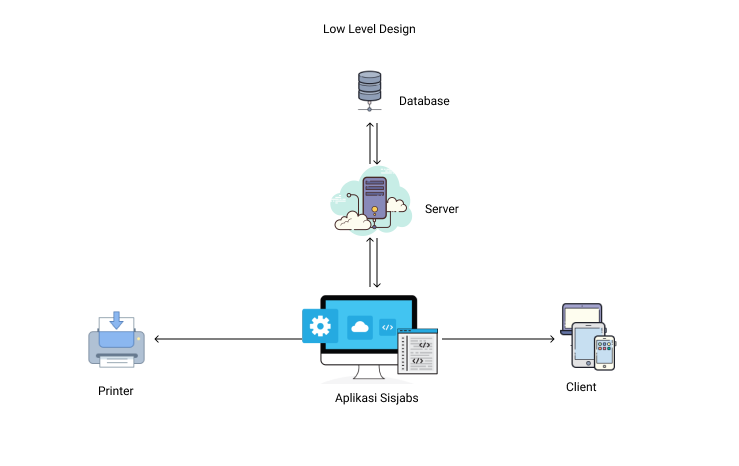
\includegraphics[width=0.9\textwidth]
	{pics/LowLevelDiagram.png}
	\caption{Low Level Design}
	\label{fig:31}
\end{figure}


\subsection{Gambaran Umum Sistem}

Aplikasi \textbf{SiPJabS : Sistem Pengawakan Jabatan Struktural di Univertias Telkom} merupakan aplikasi berbasis web yang memudahkan bagi perusahaan dalam pencarian seorang kandidat atau posisi yang kosong. Dalam pembuatan aplikasi ini dibutuhkan fitur \textit{filtering} yang digunakan untuk pencarian kandidat baru, yang sesuai dengan ketentuan yang sudah ditetapkan oleh perusahaan. Sistem \textit{filtering} dapat dilakukan setiap saat, untuk menggantikan pekerjaan lama yang telah berhenti dikarenakan pensiun, meninggal, mengundurkan diri atau diberhentikan karena suatu kebijakan tertentu.

Data-data pegawai yang berada di Universitas Telkom dapat dilihat dan data tersebut bersifat rahasia. Sehingga aplikasi ”\textbf{SiPJabS : Sistem Pengawakan Jabatan Struktural di Universitas Telkom}” hanya dapat diakses oleh orang tertentu. Aplikasi ini terdapat satu \textit{user} yang dapat mengelola proses \textit{filtering} dan satu \textit{admin} yang mengelola infrastruktur \textit{database} dan proyek \textit{server} serta jaringan.  

Sistem \textit{filtering} pada apliaksi ini terbagi menjadi dua bagian, yang pertama merupakan \textit{fitering} secara umum dengan isi \textit{form} seperti jabatan minimal dan masa kerja. Yang kedua merupakan \textit{filtering} secara khusus, dimana \textit{user} dapat mencari kandidat dengan syarat yang lebih spesifik lagi untuk dijadikan pilihan, kemudian akan terdapat beberapa nama kandidat, apabila sudah menentukan pilihan dapat menekan tombol button pada nama yang akan dipilih dan akan masuk dalam \textit{cart} kandidat.

Apabila proses pencarian kandidat sudah ditemukan dengan salah satu proses \textit{filtering} yang sudah dijelaskan diatas maka, proses selanjutnya akan masuk dalam pembuatan berita acara dan dapat dicetak berupa file pdf.  

\subsection{Target Pengguna Aplikasi}

Aplikasi \textbf{SiPJabS} memiliki beberapa target pengguna diantaranya sebagai berikut :

\begin{enumerate}
\item User \\
User merupakan pegawai Direktorat Sumber Daya Manusia Universitas Telkom yang membutuhkan kandidat dengan proses \textit{filtering} untuk mengisi posisi yang kosong atau digantikan.

\item Admin \\
Admin merupakan pegawai Direktorat Pusat Teknologi Informasi Universitas Telkom yang mengelola dan menyediakan data untuk proses filtering.
\end{enumerate}

\subsection{Spesifikasi Target Perangkat}

Spesifikasi dari target perangkat untuk mengakses aplikasi SiPJabS adalah sebagai berikut : 

\begin{enumerate}

\item Komputer atau laptop yang terhubung dengan koneksi internet dan dapat membuka \textit{browser}.

\item	\textit{Smartphone} atau tablet yang terhubung dengan koneksi internet dan dapat membuka \textit{browser}.
\end{enumerate}

\subsection{Diagram Alir Aplikasi}
\blindtext \\

%-----------------------------------------------------------------------------%
\section{Kebutuhan Pengembangan Sistem}
%-----------------------------------------------------------------------------%

Dalam membangun sistem, hal-hal yang dibutuhkan dalam mengembangkan aplikasi \textbf{SiPJabS} ini adalah sebagai berikut :

\subsection{Kubutuhan Perangkat Keras (Hardware) }

\textit{Hardware} yang dibutuhkan dalam perancangan dan pembuatan aplikasi SiPJabs
adalah sebagai berikut :


\begin{table}[H]
	\centering
	\caption{Tabel Kebutuhan Hardware}
	\begin{tabular}{ | c | l | l | }
		\hline
		No. & Perangkat Keras & Spesifikasi \\
		\hline
		\multirow{5}{*}{1} & \multirow{5}{*}{Laptop MSI GL62M} & Processor : Intel Core i7-7700HQ \\
		& & Operating sistem : Windows 10 Education \\
		& & RAM : 8 GB \\
		& & Storage : 128 GB SSD + 1 TB Hardisk \\
		& & Graphics Card :  nVidia Geforce GTX 1050 \\
		
		
		\hline
		
		\multirow{5}{*}{2} & \multirow{5}{*}{Laptop HP Pavilion x360} & Processor : Intel Core i3-6100U \\
		& & Operating sistem : Windows 10 Home \\
		& & RAM : 12 GB \\
		& & Storage : 500 GB Hardisk\\
		& & Graphics Card : Intel HD 520 Graphics \\
		\hline
	\end{tabular}
\end{table}



\subsection{Kebutuhkan Perangkat Lunak (Software)}

\textit{Software} yang dibutuhkan dalam perancangan dan pembuatan aplikasi SiPJabs
adalah sebagai berikut :

\begin{table}[H]
	\centering
	\caption{Tabel Kebutuhan Software}
	\begin{tabular}{ | c | l | p{65mm} | }
		\hline
		No. & Software & Kegunaan \\
		\hline
		
		1 & Visual Studio Code & Text editor untuk menuliskan \textit{coding} aplikasi \\
				
		\hline
		
		2 & XAMPP & Sebagai server yang berdiri sendiri, yang terdiri atas program Apache HTTP Server, MySQL database, dan penerjemah bahasa yang ditulis dengan bahasa pemrograman PHP dan Perl \\
		
		\hline
		
		3 & IBM Rational System Architect  & Sebuah software untuk mendesain rancangan sistem aplikasi \\
		
		\hline
		
		4 & Figma & Untuk mendesai user interface secara online \\
		
		
		\hline
		
		5 & Microsoft Office Word & Untuk membuat dokumen dan laporan \\
		
		\hline
		
		6 & TexStudio & Untuk membuat laporan dalam latex \\
		
		\hline
		
		7 & Adobe Premier Pro & Editing vidio demo dan vidio promosi \\
		
		\hline
		
		8 & Brave dan Mozila Firefox & Web browser \\
		
		\hline
	\end{tabular}
\end{table}

\subsection{Kebutuhan Hosting}

\textit{Hosting} yang dibutuhkan dalam perancangan dan pembuatan aplikasi SiPJabs
adalah sebagai berikut :

\begin{table}[H]
	\centering
	\caption{Tabel Kebutuhan Hosting}
	\begin{tabular}{ | c | l | l | }
		\hline
		No. & Server & Spesifikasi \\
		\hline
		\multirow{5}{*}{1} & \multirow{5}{*}{Server Indonesia} & Storage : 2 GB \\
		& & RAM : 1 GB \\
		& & Bandwith : Unlimited \\
		& & Processor : 1 Core \\
		& & Domain : my.id  \\
	
		\hline
	\end{tabular}
\end{table}

%-----------------------------------------------------------------------------%
\section{Perancangan Model Program}
%-----------------------------------------------------------------------------%
\blindtext \\

\subsection{Use Case Diagram}

\begin{figure}
	\centering
	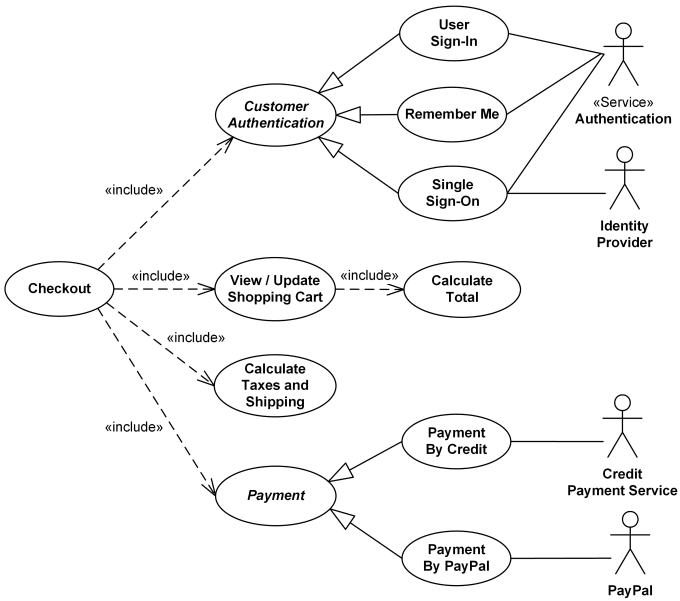
\includegraphics[width=0.9\textwidth]
	{pics/use-case-example.png}
	\caption{Online shopping UML use case diagram example}
	\label{fig:32}
\end{figure}

\subsection{Use Case Skenario}

%-----------------------------------------------------------------------------%
\section{Perancangan Aplikasi}
%-----------------------------------------------------------------------------%
Dalam perancangan aplikasi SiPJabS diperlukan perancangan antar muka dan perancangan design level tinggi. Perancangan antar muka akan menjelaskan gambaran awal  developer sebelum masuk pada bagian front-end.  Sedangkan perancangan design level tinggi berguna untuk mengingatkan developer tentang sistem kerja pada aplikasi yang akan dibuat.


\subsection{Perancangan Antar Muka}
Pada tahap kebutuhan antar muka terdapat gambaran mengenai aplikasi SiPJabS: Sistem Pengawakan Jabatan Struktural, berikut merupakan mockup dari aplikasi SiPJabS yang sudah dibuat.

\subsubsection{Perancangan Antar Muka Admin}

\begin{table}
	\caption{Tabel Perancangan Antar Muka Admin}
	\centering
	\begin{tabular}{ | c | c | p{35mm} |}
		\hline 
		\textbf{No} & \textbf{Gambar} &  \textbf{Keterangan} \\ 
		\hline
		
		1. & \raisebox{-\totalheight}{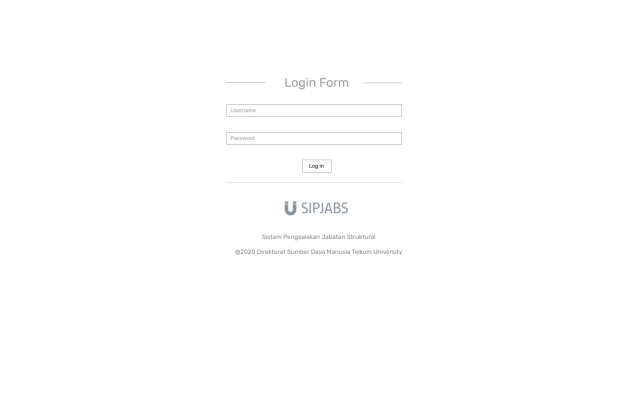
\includegraphics[width=0.6\textwidth, height=60mm]{pics/admin/login.jpg}} 
		& Halaman login merupakan tampilan awal apabila admin membuka aplikasi SiPJabS , admin dapat menginputkan username dan password untuk melakukan login. \\
	
		\hline
		
		2. & \raisebox{-\totalheight}{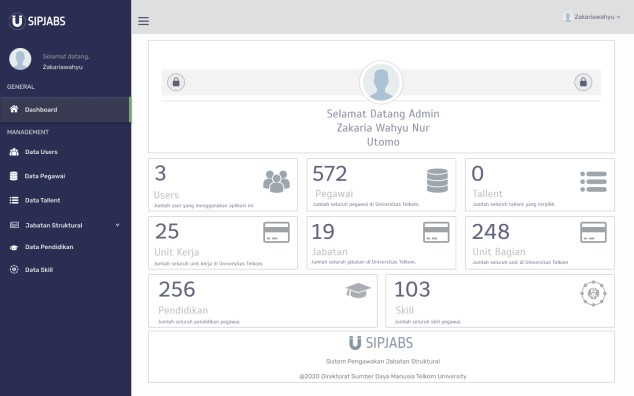
\includegraphics[width=0.6\textwidth, height=60mm]{pics/admin/dashboard.jpg}} 
		& Didalam dashboard admin terdapat jumlah users dari aplikasi SiPJabS, jumlah pegawai di Universitas Telkom, tallent yang sudah dipilih, unit kerja, jabatan, unit bagian, pendidikan dan skill yang dimiliki para pegawai  Universitas Telkom. \\
		\hline

	\end{tabular}
\end{table}


\begin{table}
	\caption{Tabel Perancangan Antar Muka Admin (1)}
	\centering
	\begin{tabular}{ | c | c | p{35mm} |}
		\hline 
		\textbf{No} & \textbf{Gambar} &  \textbf{Keterangan} \\ 
		\hline
		
		3. & \raisebox{-\totalheight}{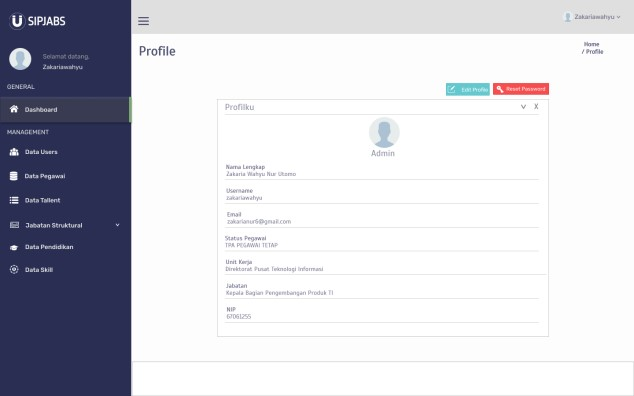
\includegraphics[width=0.6\textwidth, height=60mm]{pics/admin/profile.jpg}} 
		& Halaman profile admin akan menampilkan data profile dari admin tersebut. Kemudian admin juga dapat mengedit profile dan mereset password.  \\
		
		\hline
		
		4. & \raisebox{-\totalheight}{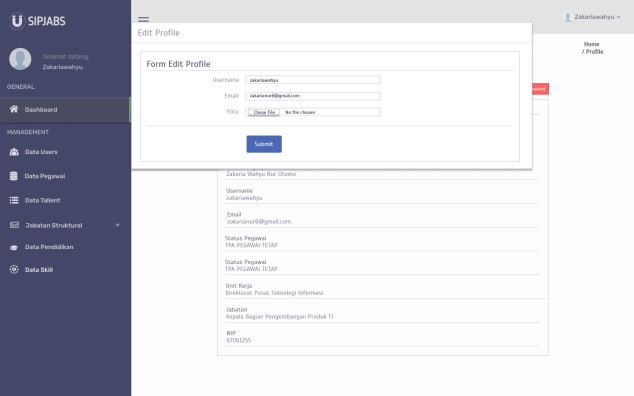
\includegraphics[width=0.6\textwidth, height=60mm]{pics/admin/editprofile.jpg}} 
		& Admin dapat mengubah username, menginputkan email, dan menambahkan foto profile.  \\
		
		\hline
		
		5. & \raisebox{-\totalheight}{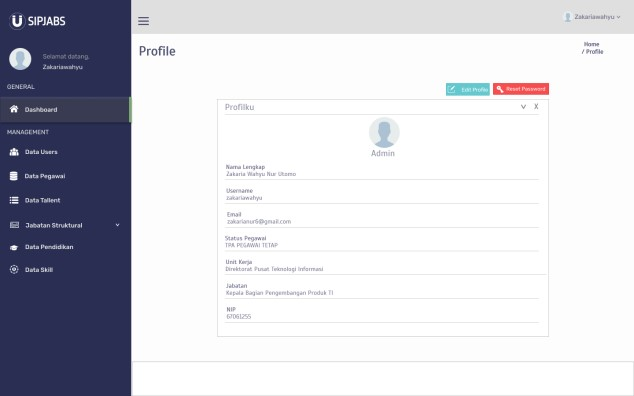
\includegraphics[width=0.6\textwidth, height=60mm]{pics/admin/profile.jpg}} 
		& Halaman profile admin akan menampilkan data dari admin tersebut. Kemudian admin juga dapat mengedit profile dan mereset password. \\
		
		\hline
		
	\end{tabular}
\end{table}

\begin{table}
	\caption{Tabel Perancangan Antar Muka Admin (2)}
	\centering
	\begin{tabular}{ | c | c | p{35mm} |}
		\hline 
		\textbf{No} & \textbf{Gambar} &  \textbf{Keterangan} \\ 
		\hline
		
		6. & \raisebox{-\totalheight}{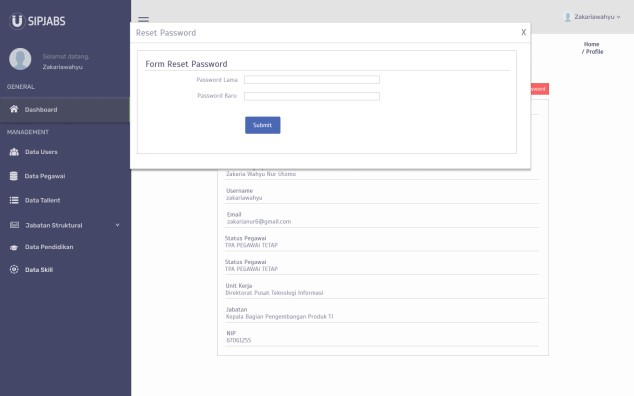
\includegraphics[width=0.6\textwidth, height=60mm]{pics/admin/resetpassword.jpg}} 
		& Admin harus menginputkan password yang lama serta yang baru, setelah itu admin dapat menyimpan. \\
		
		\hline
		
		7. & \raisebox{-\totalheight}{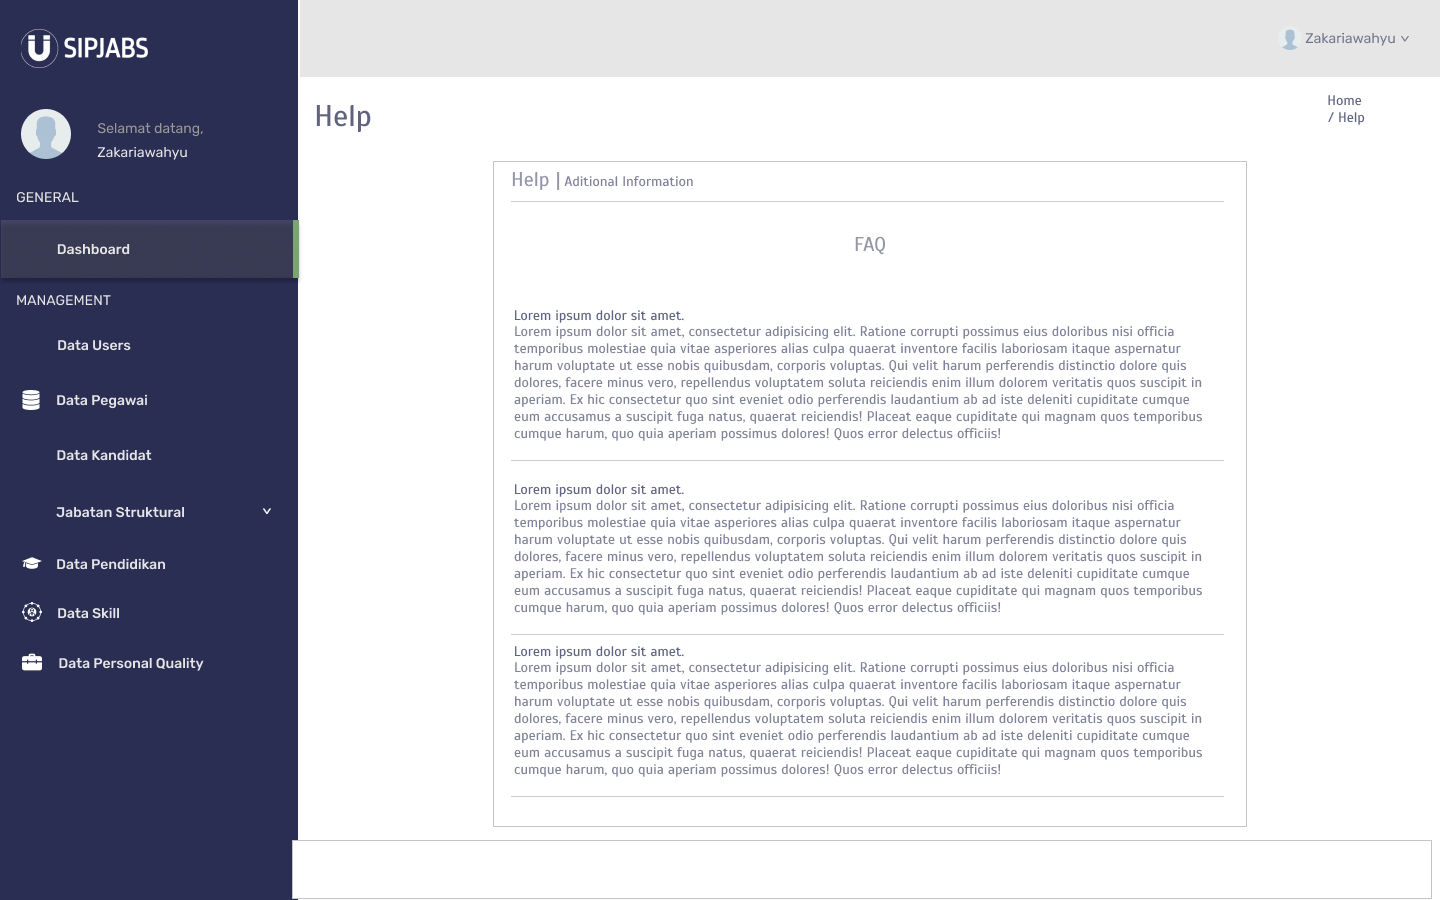
\includegraphics[width=0.6\textwidth, height=60mm]{pics/admin/help.png}} 
		& Halaman help berisi infomasi tentang aplikasi. \\
		
		\hline
		
		8. & \raisebox{-\totalheight}{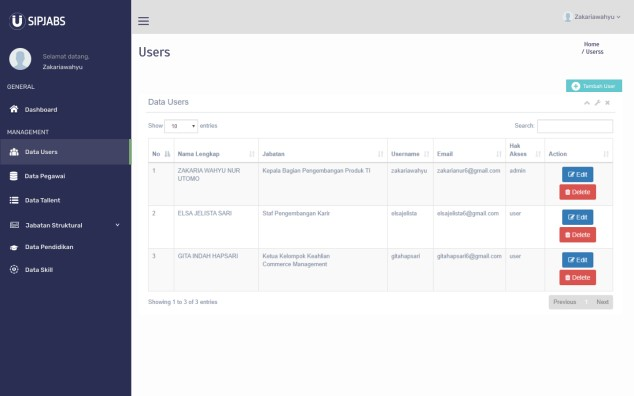
\includegraphics[width=0.6\textwidth, height=60mm]{pics/admin/datausers.jpg}} 
		& Halaman data user akan menampilkan nama-nama yang dapat mengakses aplikasi SiPJabS sebagai admin dan user. \\
		
		\hline
		
	\end{tabular}
\end{table}

\begin{table}
	\caption{Tabel Perancangan Antar Muka Admin (3)}
	\centering
	\begin{tabular}{ | c | c | p{35mm} |}
		\hline 
		\textbf{No} & \textbf{Gambar} &  \textbf{Keterangan} \\ 
		\hline
		
		9. & \raisebox{-\totalheight}{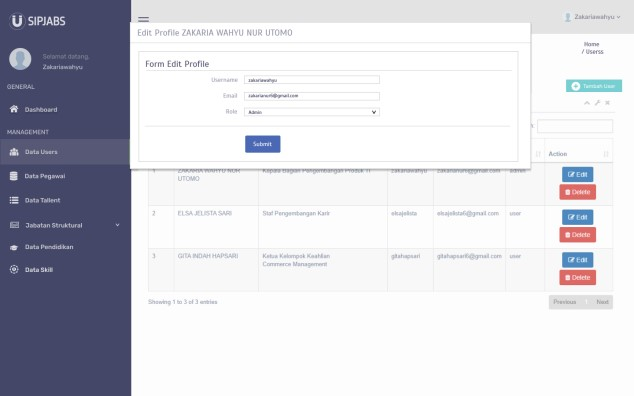
\includegraphics[width=0.6\textwidth, height=60mm]{pics/admin/editdatausers.jpg}} 
		& Pada halaman ini admin dapat mengedit username, email, dan role sebagai admin atau user. \\
		
		\hline
		
		10. & \raisebox{-\totalheight}{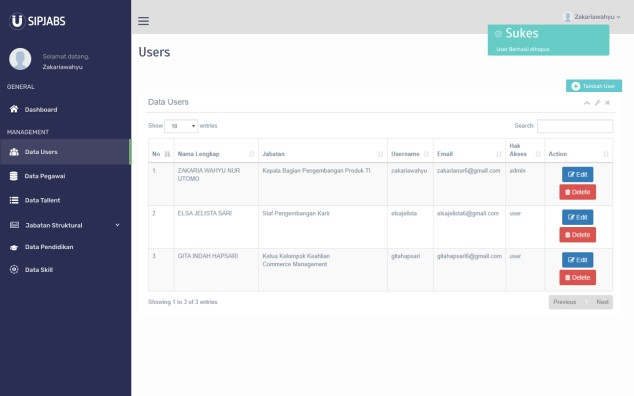
\includegraphics[width=0.6\textwidth, height=60mm]{pics/admin/hapususers.jpg}} 
		&Admin dapat menghapus data user apabila user tersebut sudah tidak bekerja pada bidangnya atau digantikan. \\
		
		\hline
		
		11. & \raisebox{-\totalheight}{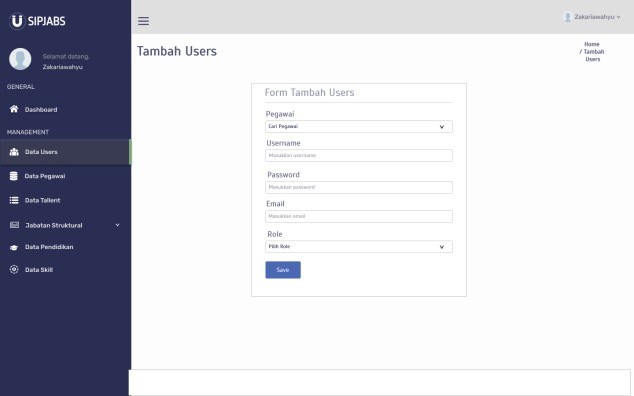
\includegraphics[width=0.6\textwidth, height=60mm]{pics/admin/tambahusers.jpg}} 
		& Admin dapat menambahkan user dengan mengisi form tambah user dan menyimpannya.. \\
		
		\hline
		
	\end{tabular}
\end{table}

\begin{table}
	\caption{Tabel Perancangan Antar Muka Admin (4)}
	\centering
	\begin{tabular}{ | c | c | p{35mm} |}
		\hline 
		\textbf{No} & \textbf{Gambar} &  \textbf{Keterangan} \\ 
		\hline
		
		12. & \raisebox{-\totalheight}{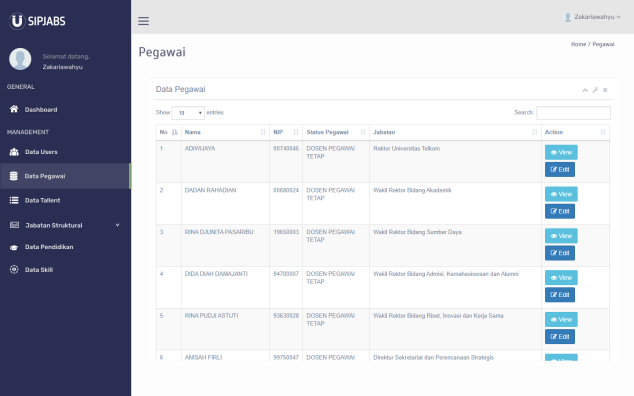
\includegraphics[width=0.6\textwidth, height=60mm]{pics/admin/datapegawai.png}} 
		& Admin dapat melihat daftar data pegawai yang ada di Universitas Telkom secara detail. \\
		
		\hline
		
		13. & \raisebox{-\totalheight}{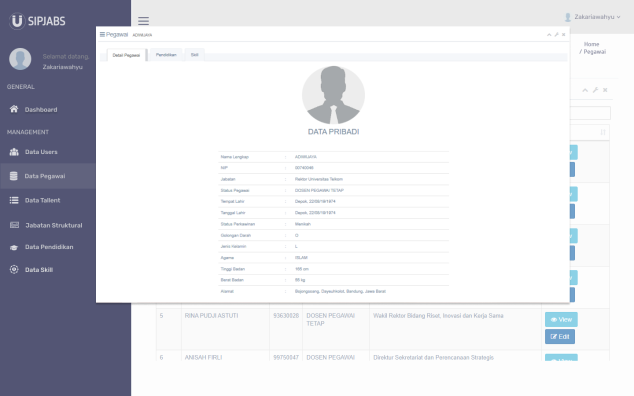
\includegraphics[width=0.6\textwidth, height=60mm]{pics/admin/viewdetailpegawai.png}} 
		&Halaman ini akan menampilkan data pribadi dari pegawai.  \\
		
		\hline
		
		14. & \raisebox{-\totalheight}{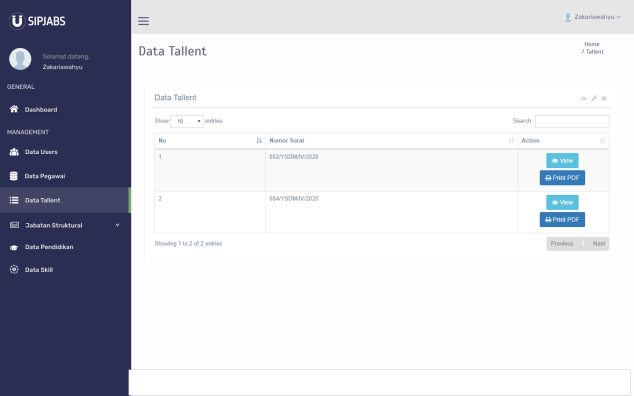
\includegraphics[width=0.6\textwidth, height=60mm]{pics/admin/datatallent.png}} 
		& Halaman ini akan menampilkan data tallent yang sudah di pilih oleh user sesuai dengan job description untuk menggantikan atau mengisi posisi yang kosong. \\
		
		\hline
		
	\end{tabular}
\end{table}

\begin{table}
	\caption{Tabel Perancangan Antar Muka Admin (5)}
	\centering
	\begin{tabular}{ | c | c | p{35mm} |}
		\hline 
		\textbf{No} & \textbf{Gambar} &  \textbf{Keterangan} \\ 
		\hline
		
		15. & \raisebox{-\totalheight}{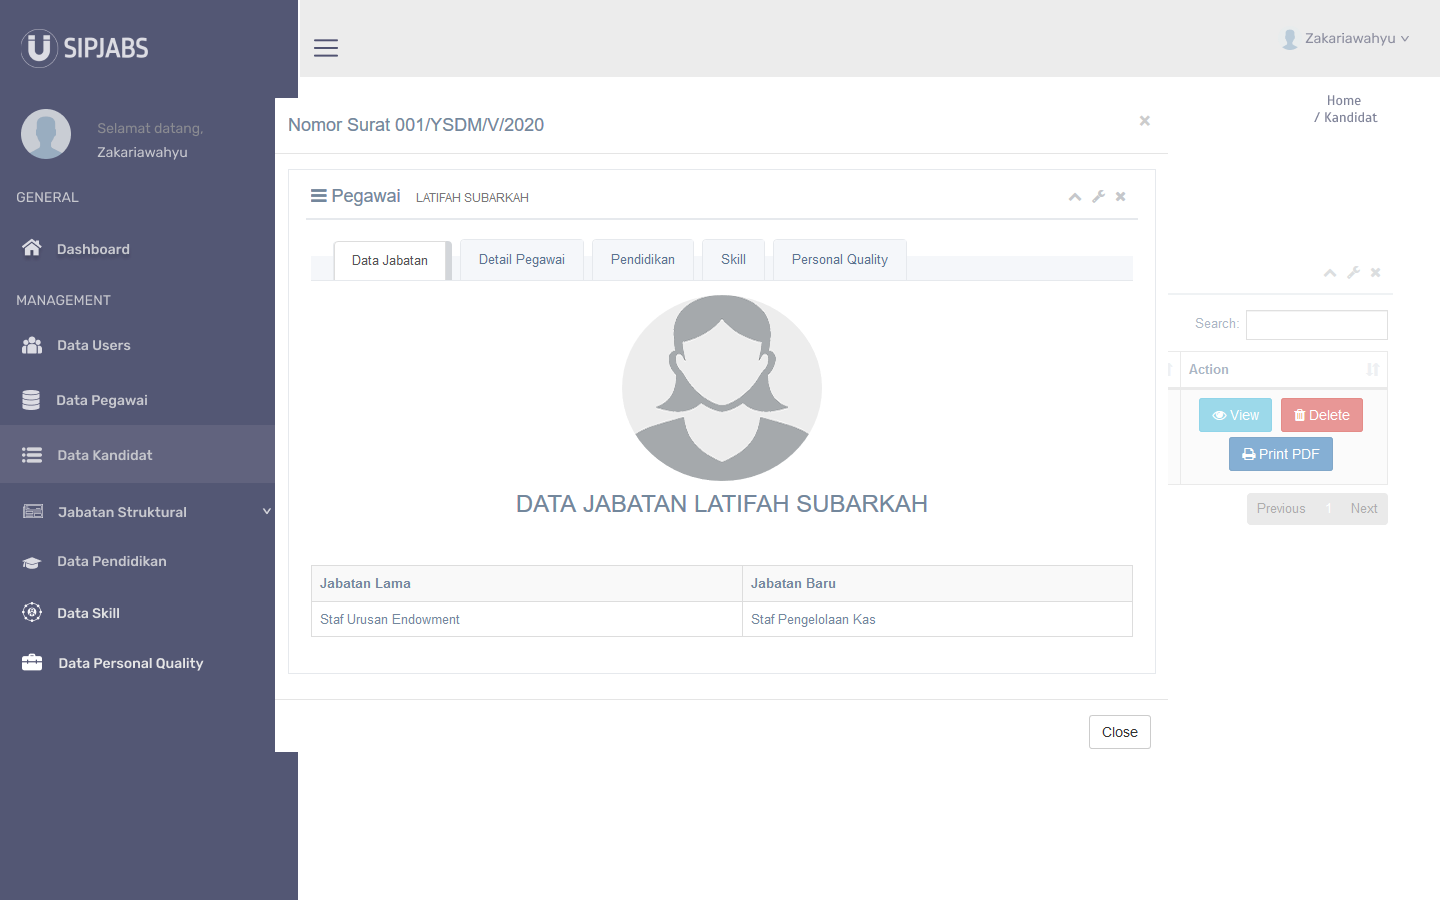
\includegraphics[width=0.6\textwidth, height=60mm]{pics/admin/viewdetailtallent.png}} 
		& Admin dapat melihat data detail tallent yang sudah dipilih. \\
		
		\hline
		
		16. & \raisebox{-\totalheight}{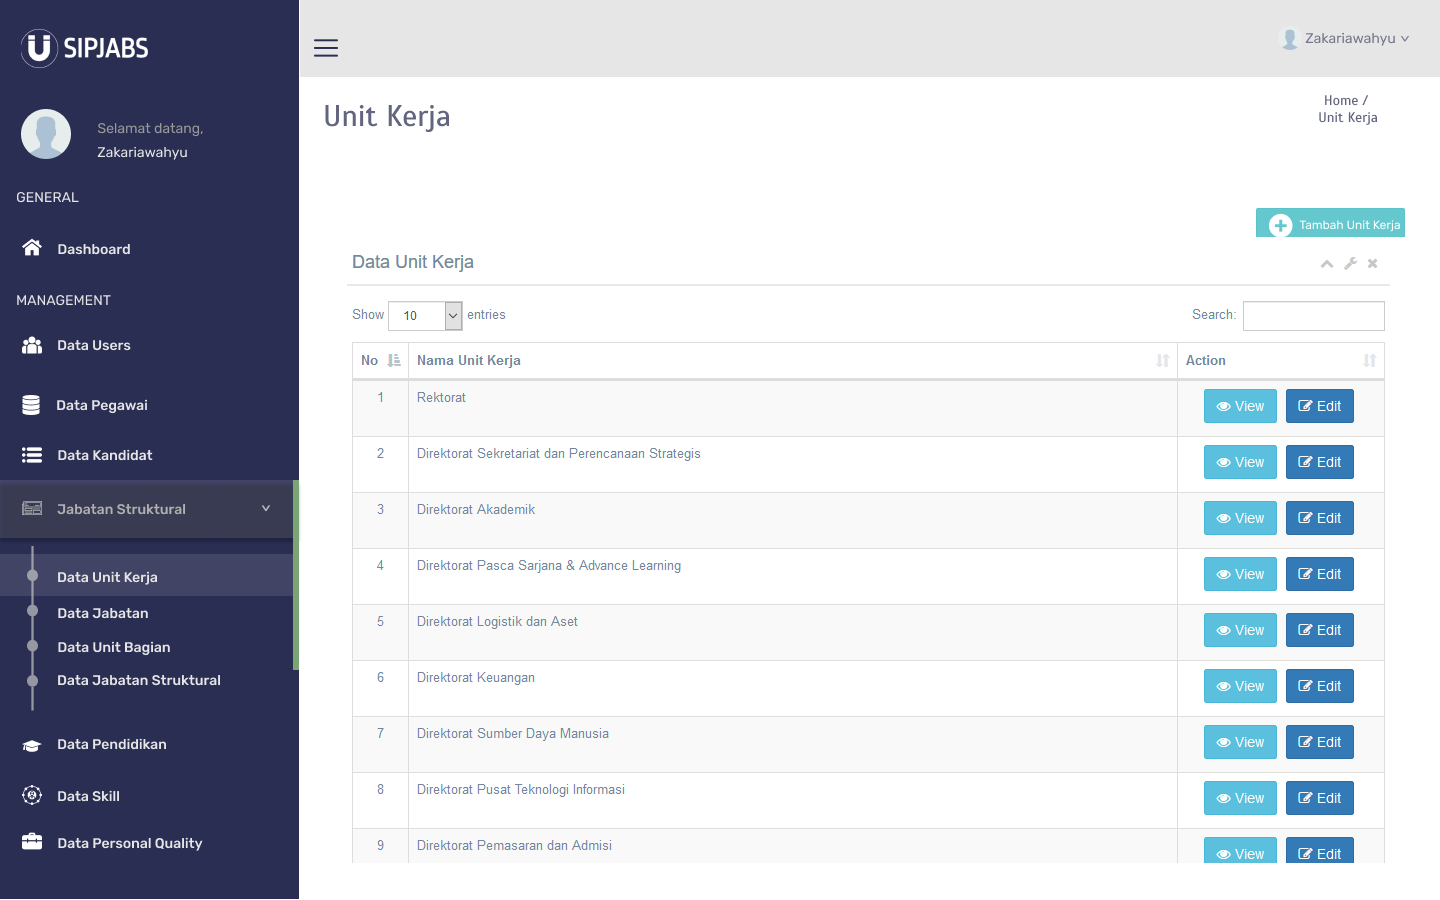
\includegraphics[width=0.6\textwidth, height=60mm]{pics/admin/dataunitkerja.png}} 
		&Halaman ini akan menunjukkan semua unit kerja dimulai dari rektorat hingga fakultas yang ada di Universitas Telkom. \\
		
		\hline
		
		17. & \raisebox{-\totalheight}{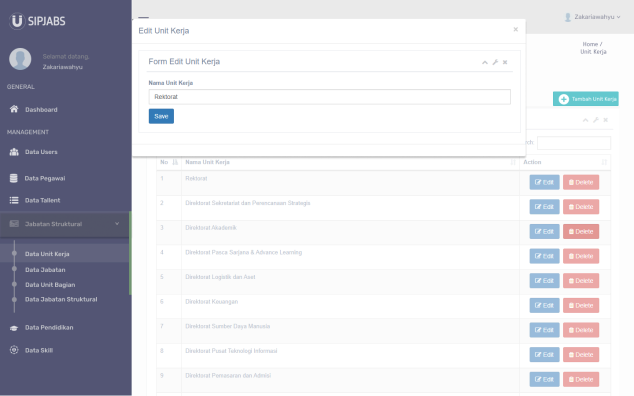
\includegraphics[width=0.6\textwidth, height=60mm]{pics/admin/editunitkerja.png}} 
		& Admin dapat mengedit form unit kerja apabila terdapat kebijakan baru. \\
		
		\hline
		
	\end{tabular}
\end{table}

\begin{table}
	\caption{Tabel Perancangan Antar Muka Admin (6)}
	\centering
	\begin{tabular}{ | c | c | p{35mm} |}
		\hline 
		\textbf{No} & \textbf{Gambar} &  \textbf{Keterangan} \\ 
		\hline
		
		18. & \raisebox{-\totalheight}{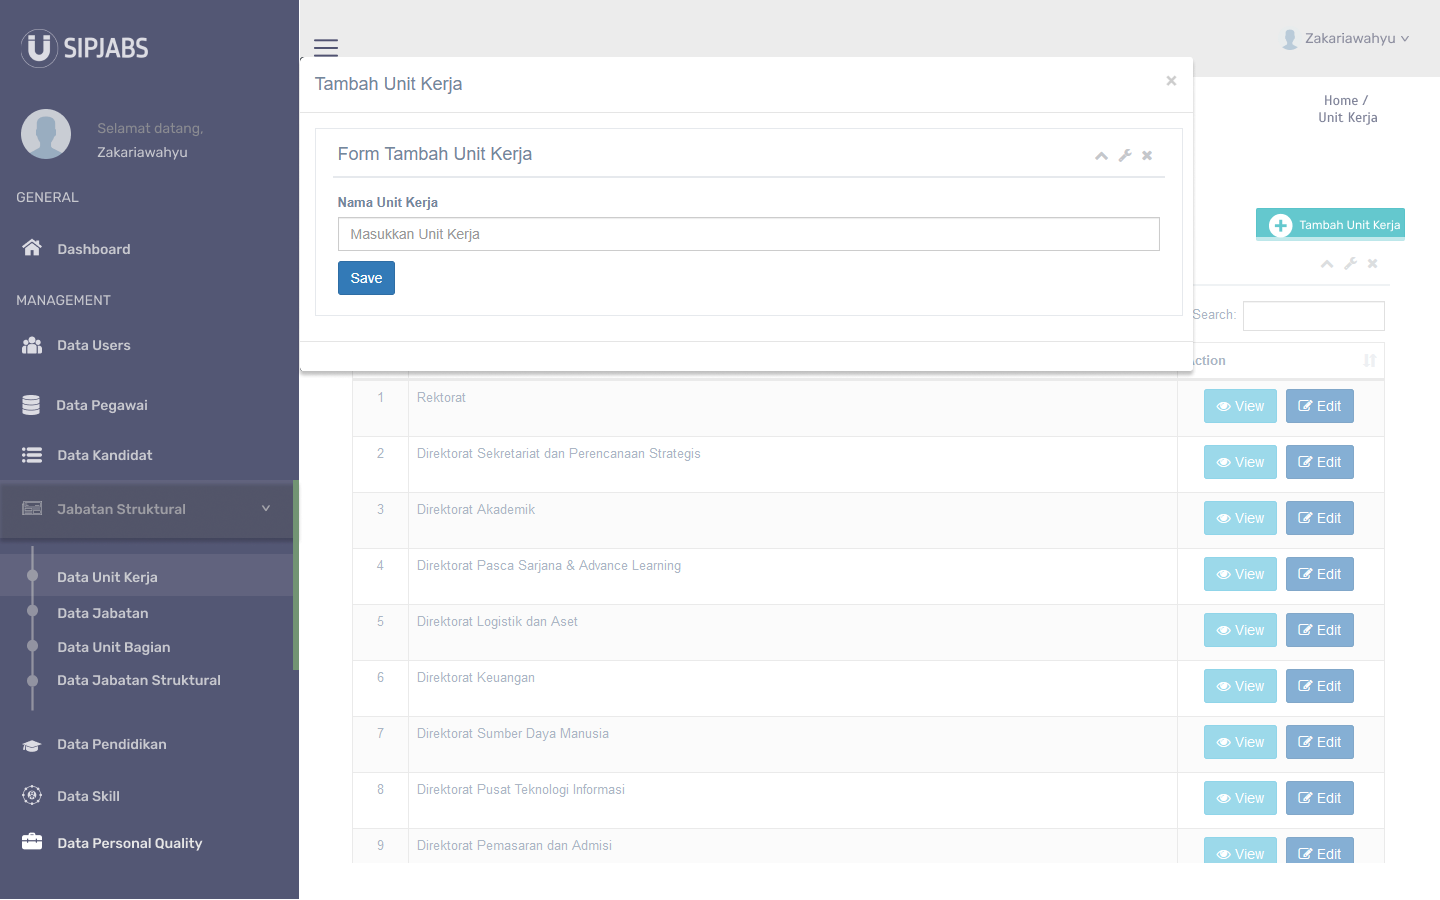
\includegraphics[width=0.6\textwidth, height=60mm]{pics/admin/tambahunitkerja.png}} 
		& Admin dapat menambahkan data unit kerja dengan mengisi form tersebut, namun harus sesuai dengan kebijakan yang telah ditetapkan. \\
		
		\hline
		
		19. & \raisebox{-\totalheight}{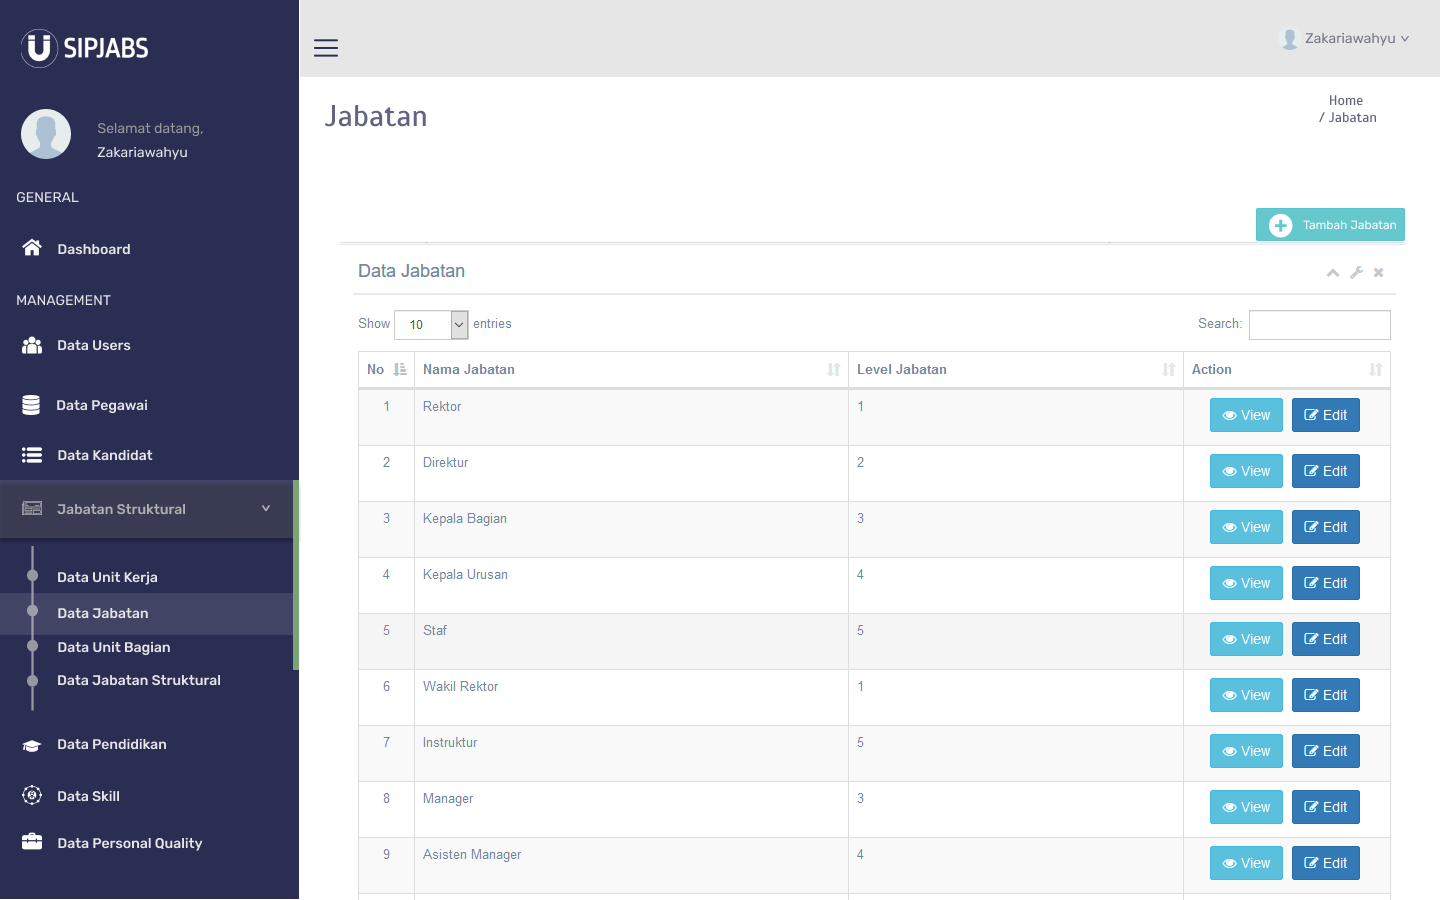
\includegraphics[width=0.6\textwidth, height=60mm]{pics/admin/datajabatan.png}} 
		&Halaman ini akan menampilkan data jabatan yang berada di Universitas Telkom \\
		
		\hline
		
		20. & \raisebox{-\totalheight}{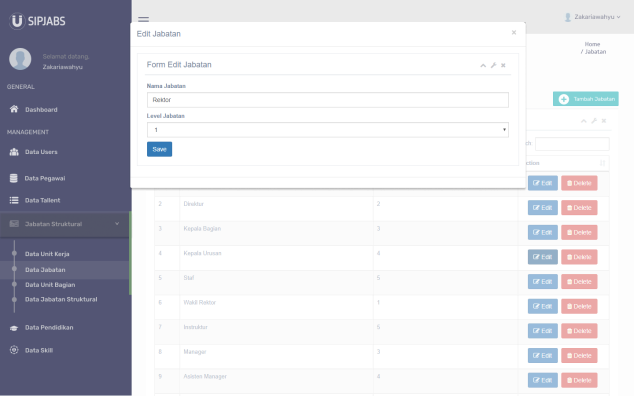
\includegraphics[width=0.6\textwidth, height=60mm]{pics/admin/editjabatan.png}} 
		& Admin dapat mengedit data jabatan sesuai dengan nama jabatan yang sudah ditetapkan. \\
		
		\hline
		
	\end{tabular}
\end{table}

\begin{table}
	\caption{Tabel Perancangan Antar Muka Admin (7)}
	\centering
	\begin{tabular}{ | c | c | p{35mm} |}
		\hline 
		\textbf{No} & \textbf{Gambar} &  \textbf{Keterangan} \\ 
		\hline
		
		21. & \raisebox{-\totalheight}{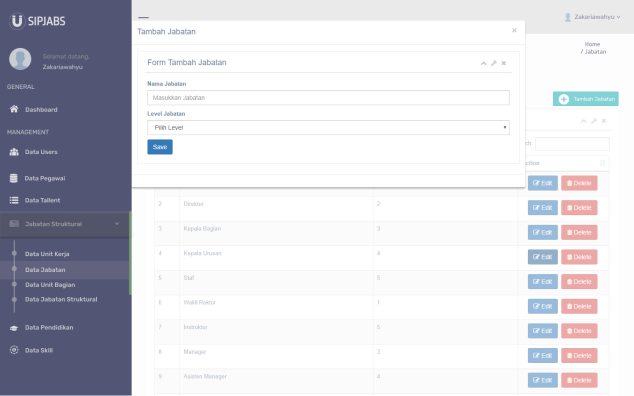
\includegraphics[width=0.6\textwidth, height=60mm]{pics/admin/tambahjabatan.png}} 
		& Admin harus melengkapi form tersebut untuk dapat menambahkan data jabatan yang baru. \\
		
		\hline
		
		22. & \raisebox{-\totalheight}{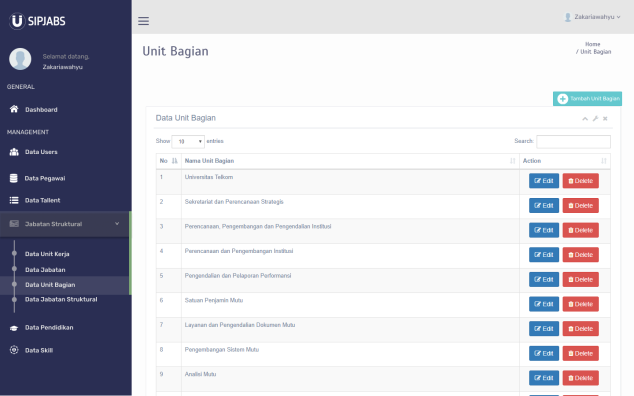
\includegraphics[width=0.6\textwidth, height=60mm]{pics/admin/dataunitbagian.png}} 
		&Halaman ini akan menampilkan satuan kerja yang terdapat di Universitas Telkom.  \\
		
		\hline
		
		23. & \raisebox{-\totalheight}{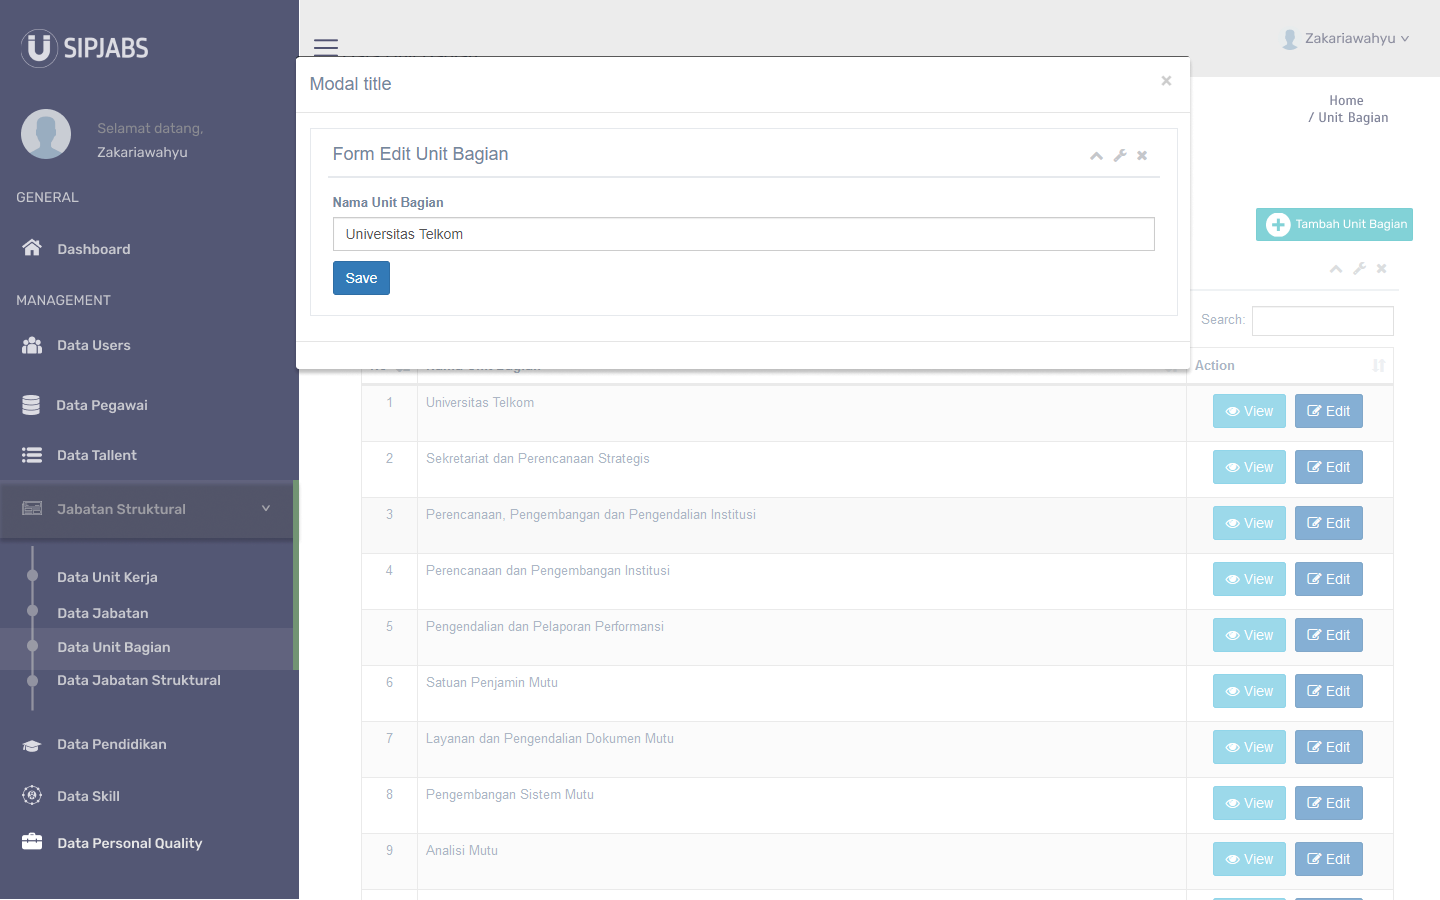
\includegraphics[width=0.6\textwidth, height=60mm]{pics/admin/editunitbagian.png}} 
		& Admin dapat mengedit data unit bagian apabila ada perubahan yang sudah ditetapkan.\\
		
		\hline
		
	\end{tabular}
\end{table}

\begin{table}
	\caption{Tabel Perancangan Antar Muka Admin (8)}
	\centering
	\begin{tabular}{ | c | c | p{35mm} |}
		\hline 
		\textbf{No} & \textbf{Gambar} &  \textbf{Keterangan} \\ 
		\hline
		
		24. & \raisebox{-\totalheight}{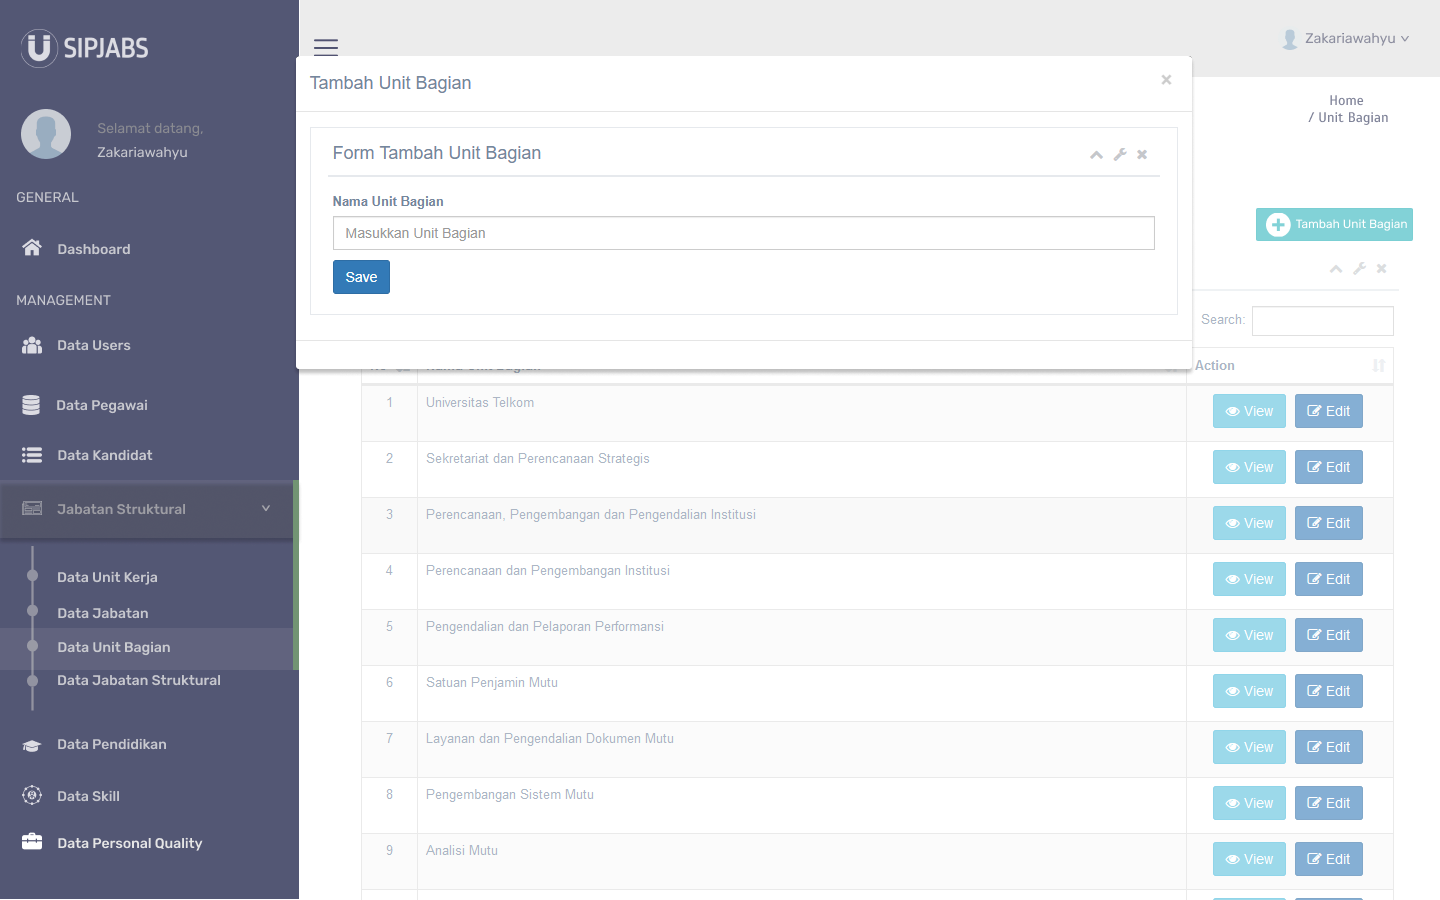
\includegraphics[width=0.6\textwidth, height=60mm]{pics/admin/tambahunitbagian.png}} 
		& Admin harus menginputkan  nama unit bagian  tersebut untuk dapat menambahkan data data unit bagian yang baru. \\
		
		\hline
		
		25. & \raisebox{-\totalheight}{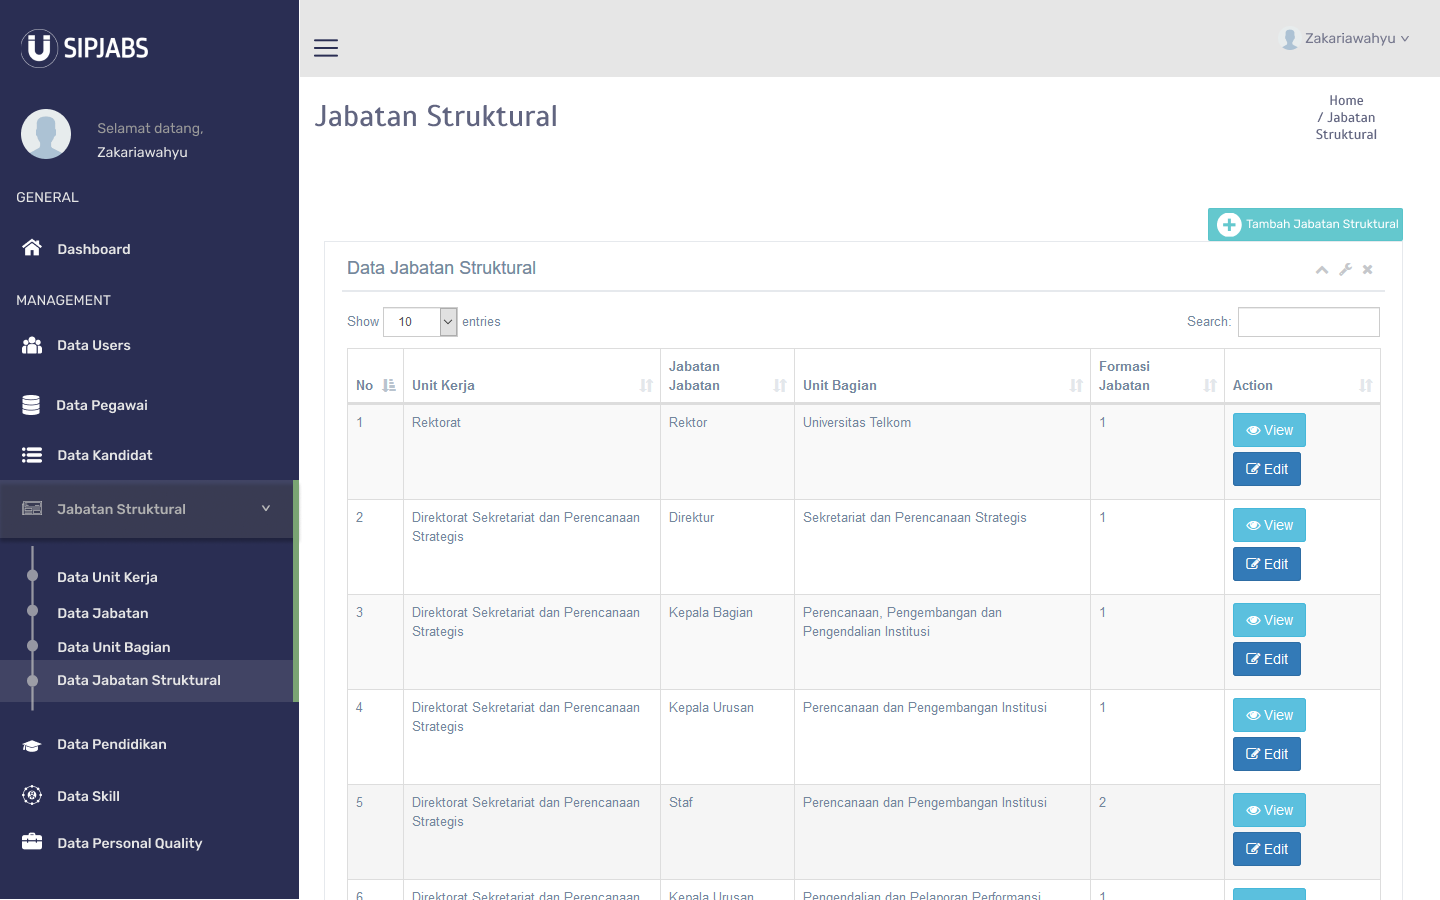
\includegraphics[width=0.6\textwidth, height=60mm]{pics/admin/datajabstruk.png}} 
		&Halaman ini menampilkan jabatan yang secara tegas ada di Universitas Telkom.  \\
		
		\hline
		
		26. & \raisebox{-\totalheight}{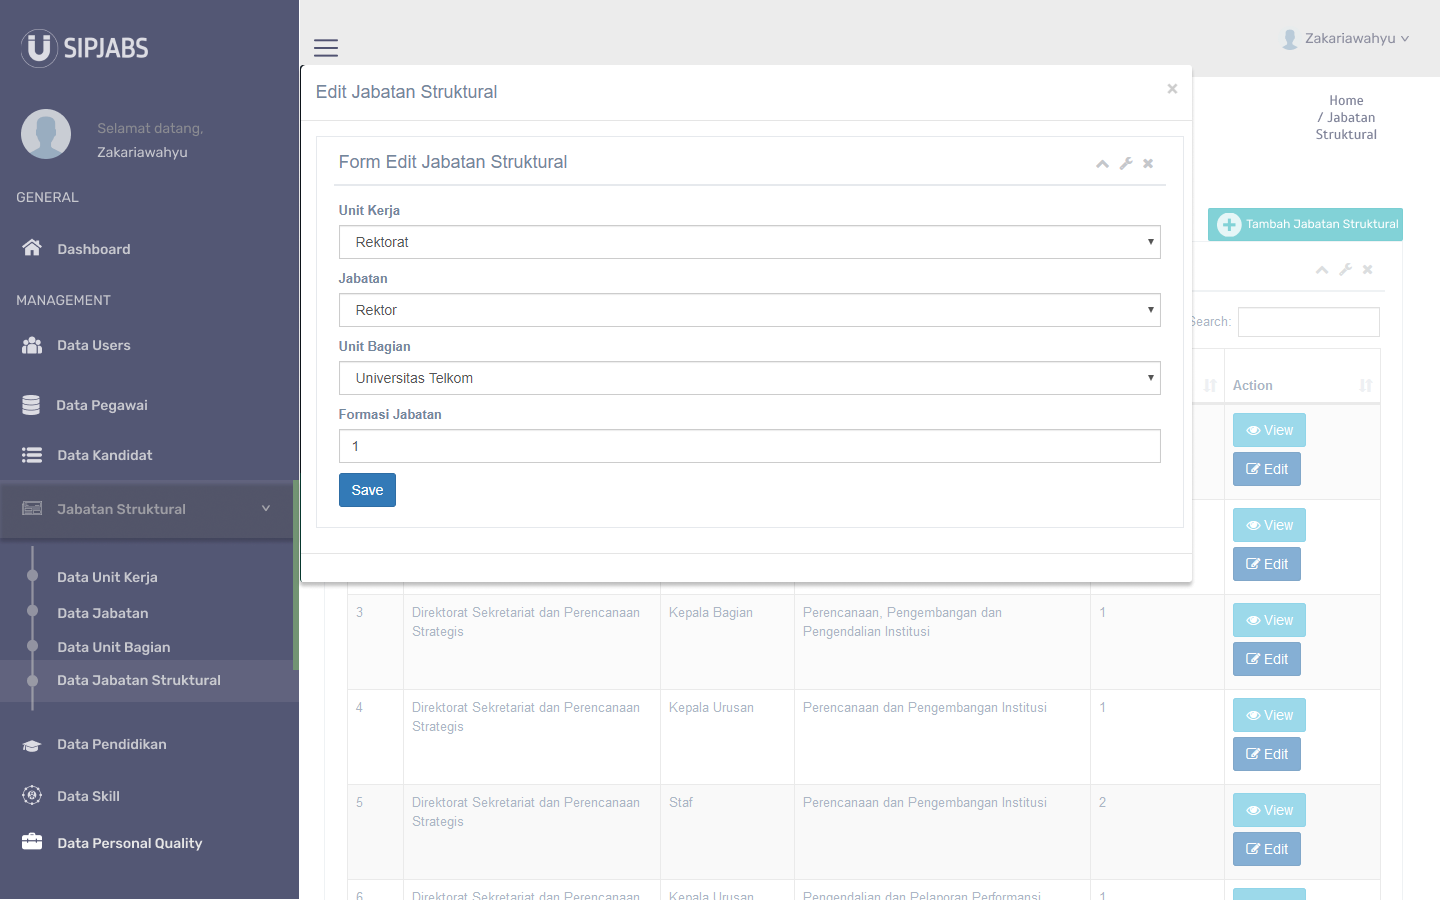
\includegraphics[width=0.6\textwidth, height=60mm]{pics/admin/editjabstruk.png}} 
		& Admin dapat mengedit data dan harus mengisi form sesuai dengan ketetapan.\\
		
		\hline
		
	\end{tabular}
\end{table}

\begin{table}
	\caption{Tabel Perancangan Antar Muka Admin (9)}
	\centering
	\begin{tabular}{ | c | c | p{35mm} |}
		\hline 
		\textbf{No} & \textbf{Gambar} &  \textbf{Keterangan} \\ 
		\hline
		
		27. & \raisebox{-\totalheight}{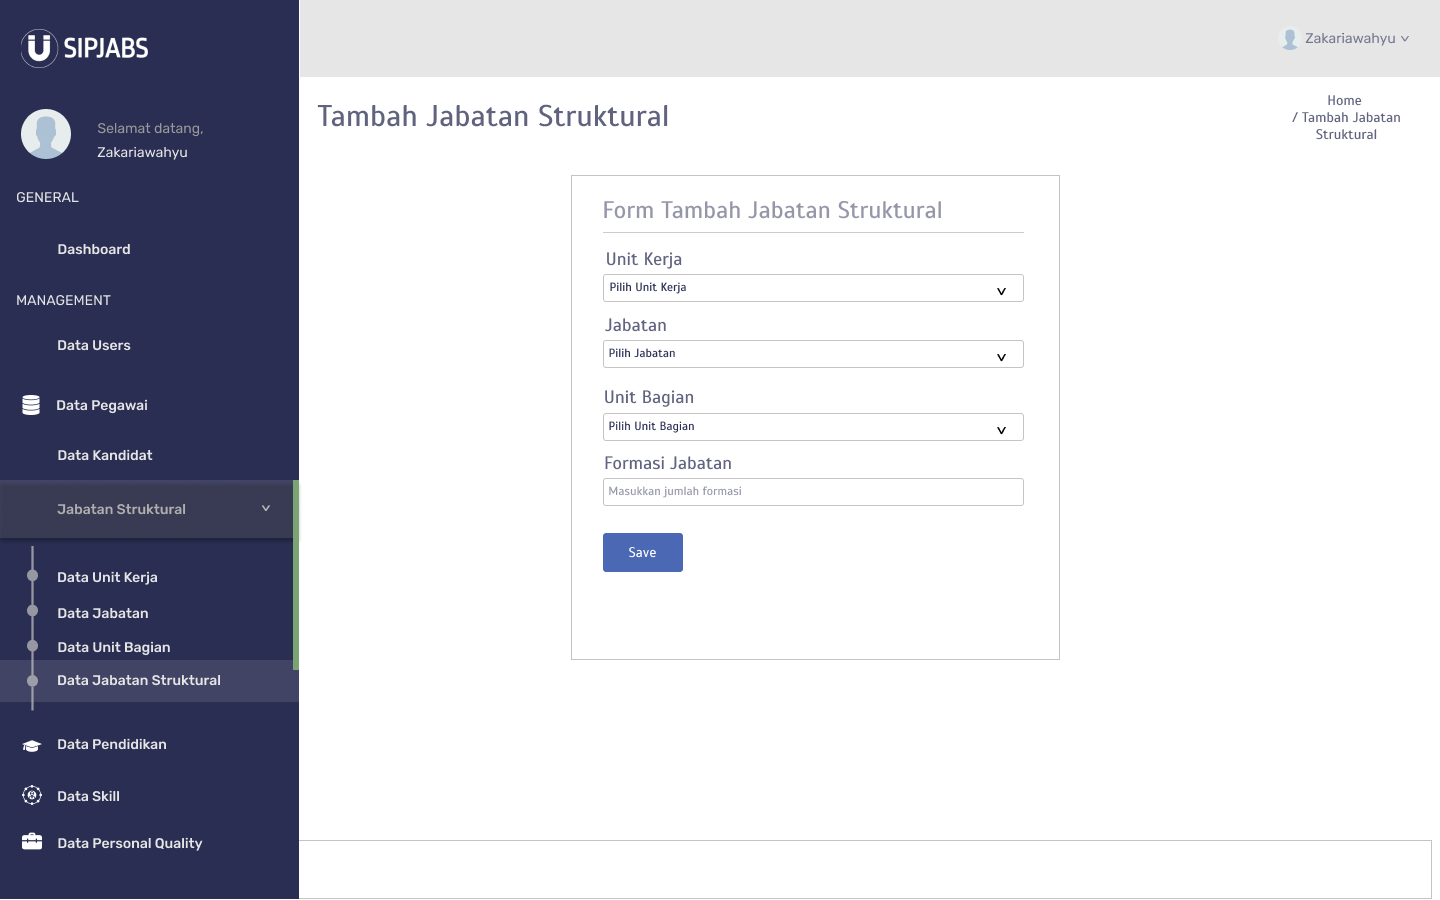
\includegraphics[width=0.6\textwidth, height=60mm]{pics/admin/tambahjabstruk.png}} 
		& Admin harus melengkapi form untuk dapat menambahkan data jabatan struktural baru yang sudah ditetapkan. \\
		
		\hline
		
		28. & \raisebox{-\totalheight}{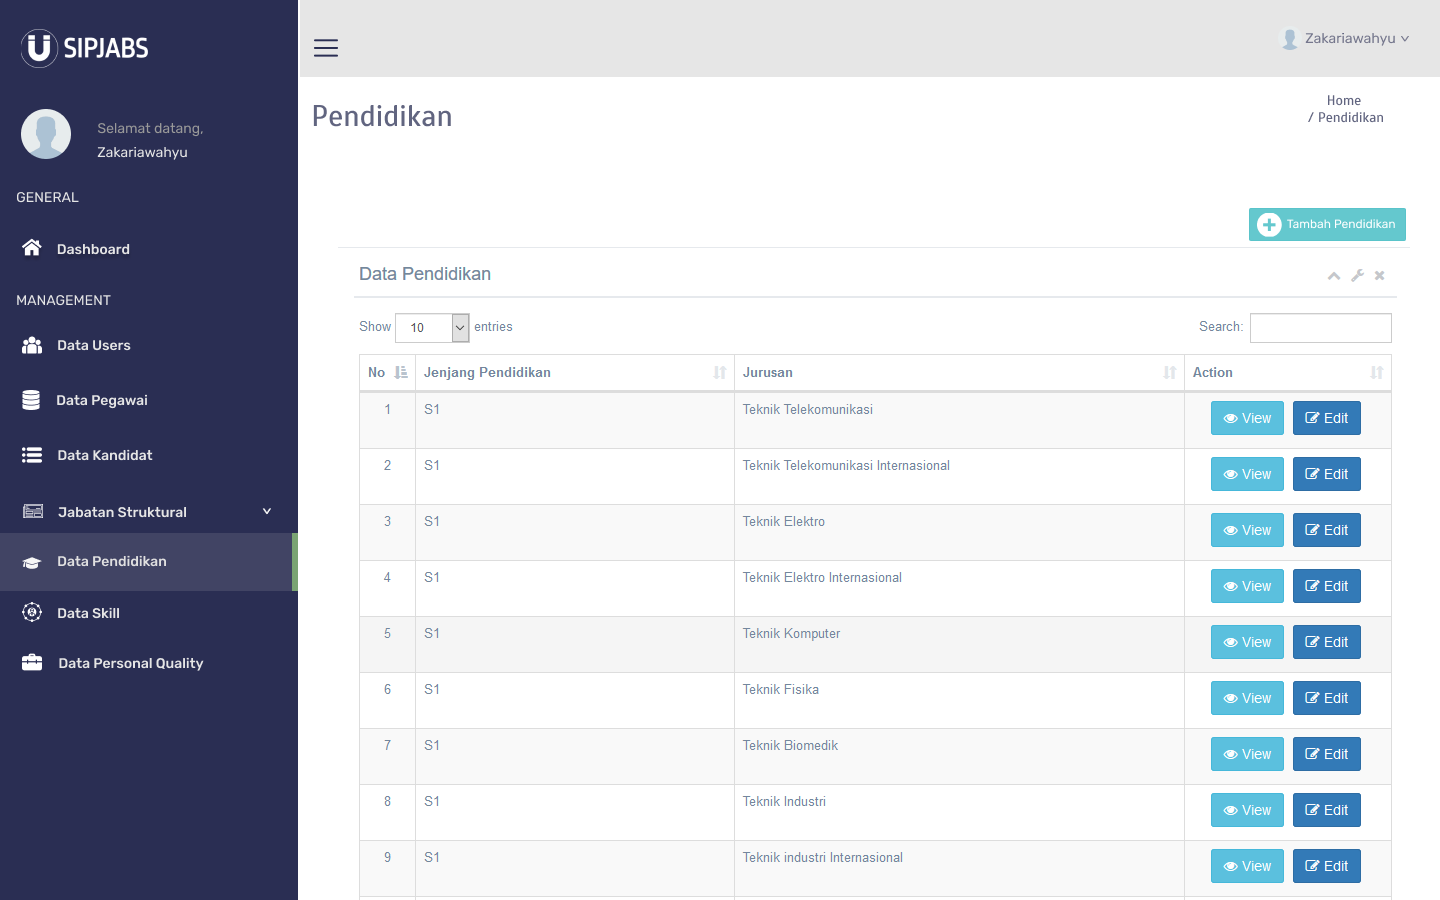
\includegraphics[width=0.6\textwidth, height=60mm]{pics/admin/datapendidikan.png}} 
		&Halaman ini akan menampilkan data pendidikan yang dimiliki pegawai Universitas Telkom.  \\
		
		\hline
		
		29. & \raisebox{-\totalheight}{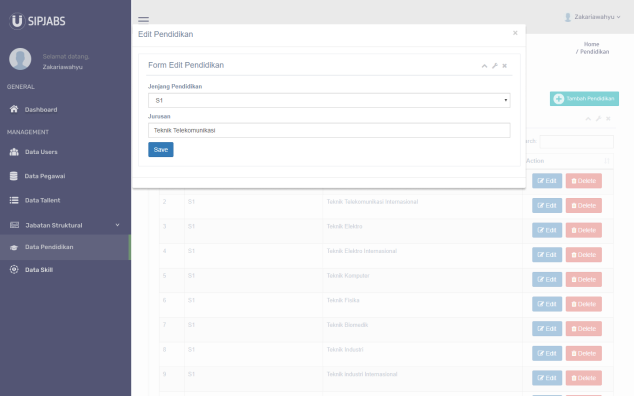
\includegraphics[width=0.6\textwidth, height=60mm]{pics/admin/editpendidikan.png}} 
		& Apabila ingin mengedit maka admin harus menginputkan jenjang pendidikan serta jurusan. \\
		
		\hline
		
	\end{tabular}
\end{table}

\begin{table}
	\caption{Tabel Perancangan Antar Muka Admin (10)}
	\centering
	\begin{tabular}{ | c | c | p{35mm} |}
		\hline 
		\textbf{No} & \textbf{Gambar} &  \textbf{Keterangan} \\ 
		\hline
		
		30. & \raisebox{-\totalheight}{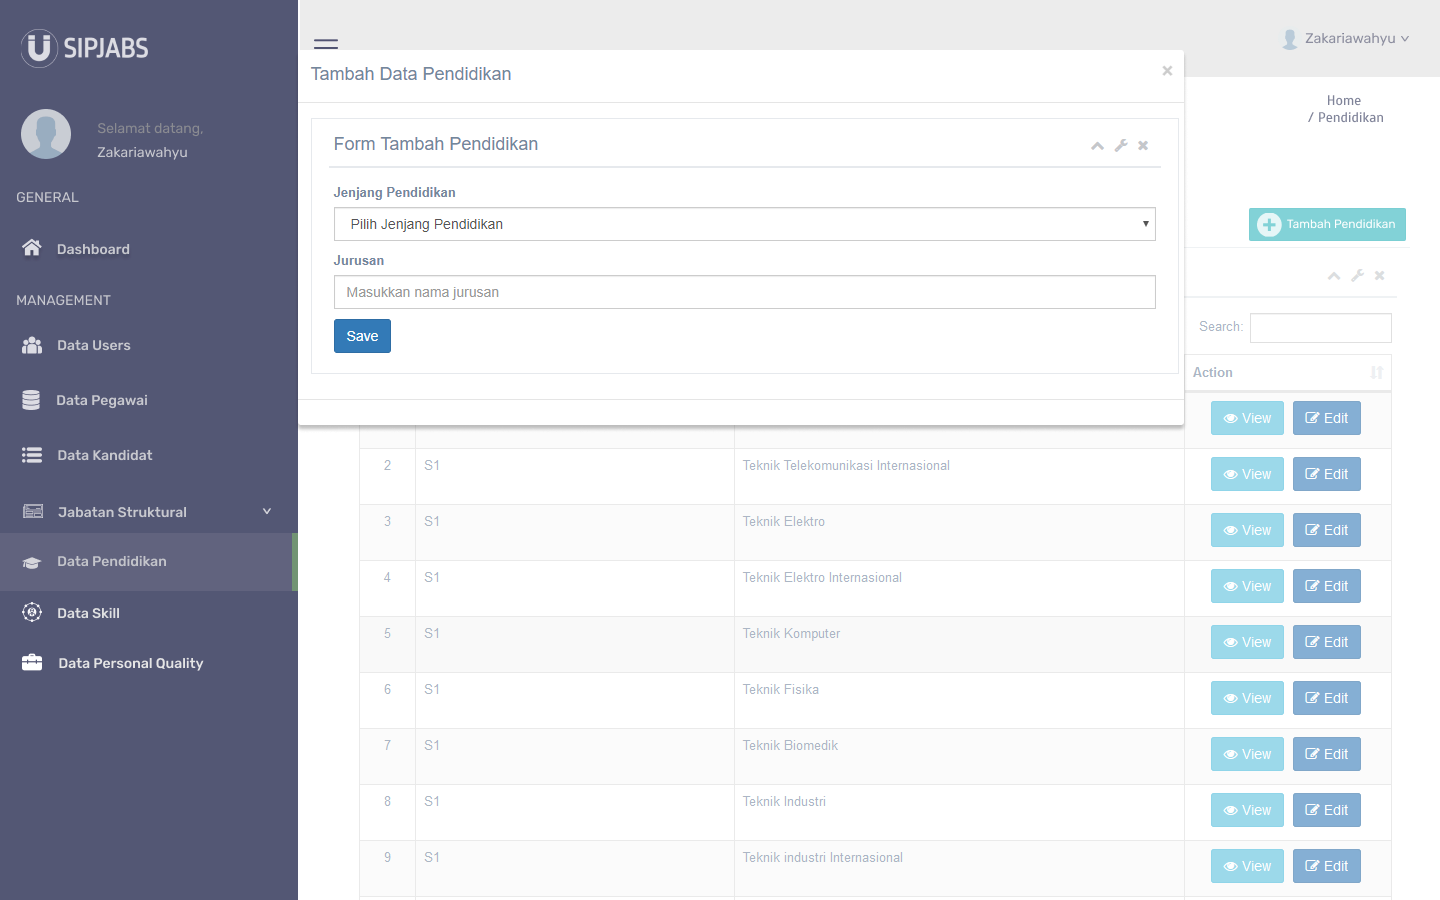
\includegraphics[width=0.6\textwidth, height=60mm]{pics/admin/tambahpendidikan.png}} 
		& Admin dapat menambahkan data pendidikan apabila belum ada data pendidikan yang dimiliki pegawai belum terinput. \\
		
		\hline
		
		31. & \raisebox{-\totalheight}{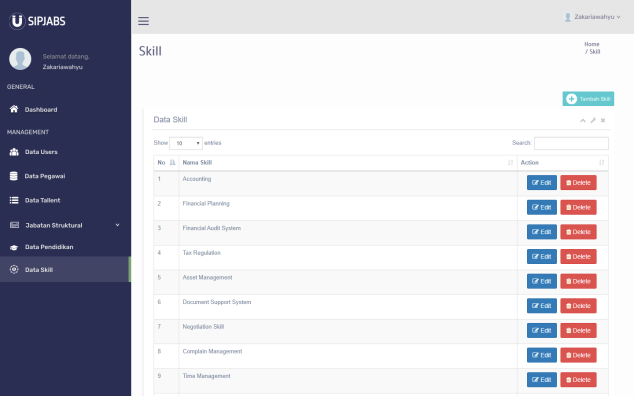
\includegraphics[width=0.6\textwidth, height=60mm]{pics/admin/dataskill.png}} 
		&Halaman ini akan menampilkan skill yang dimiliki pegawai Universitas Telkom untuk menunjang pekerjaan.  \\
		
		\hline
		
		32. & \raisebox{-\totalheight}{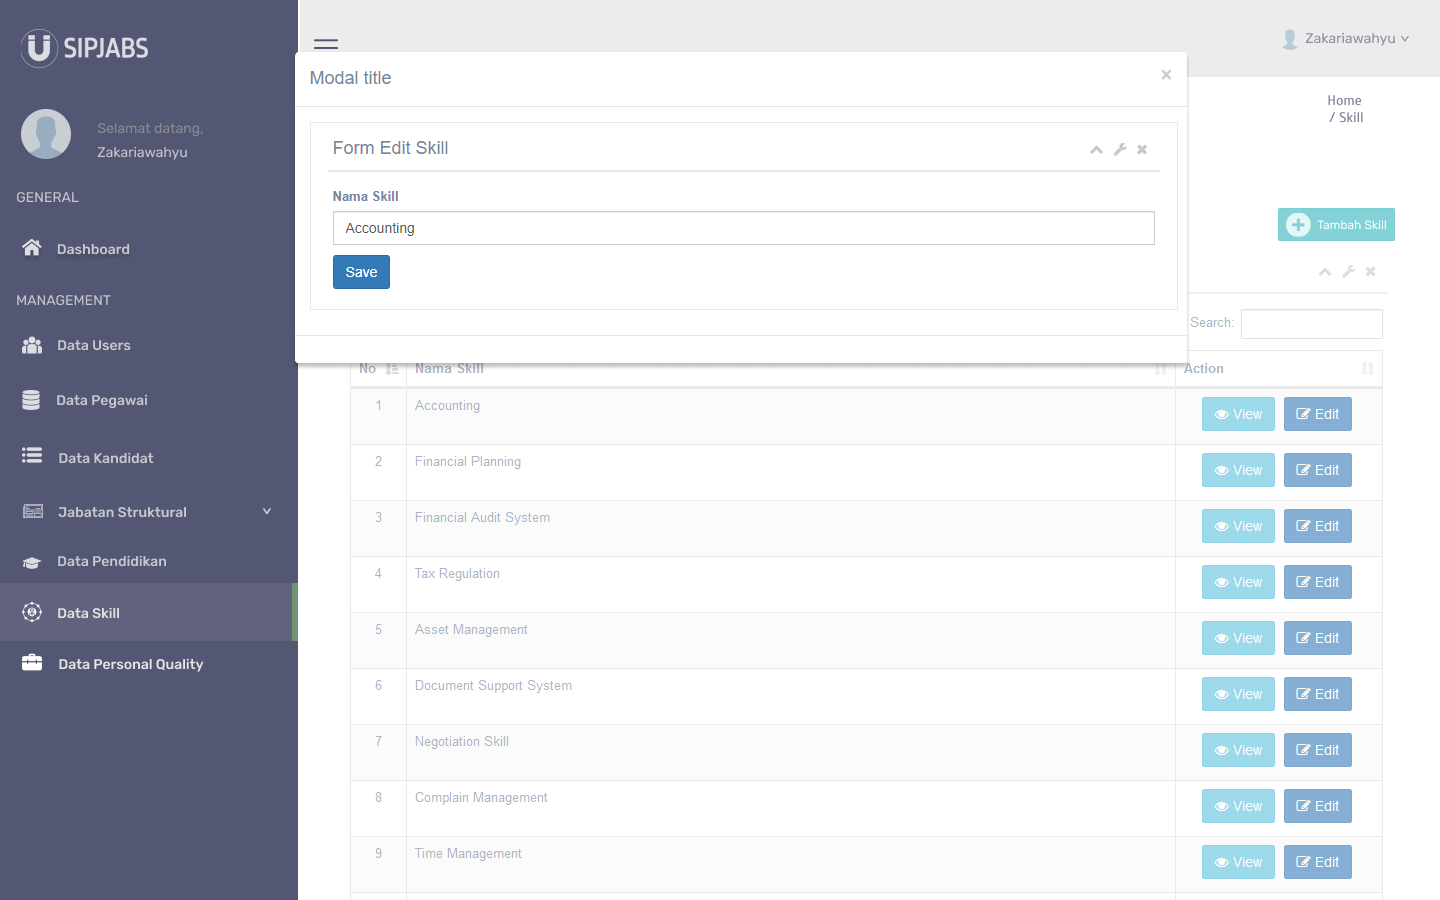
\includegraphics[width=0.6\textwidth, height=60mm]{pics/admin/editskill.png}} 
		& Admin dapat mengedit data skill. \\
		
		\hline
		
	\end{tabular}
\end{table}

\begin{table}
	\caption{Tabel Perancangan Antar Muka Admin (11)}
	\centering
	\begin{tabular}{ | c | c | p{35mm} |}
		\hline 
		\textbf{No} & \textbf{Gambar} &  \textbf{Keterangan} \\ 
		\hline
		
		33. & \raisebox{-\totalheight}{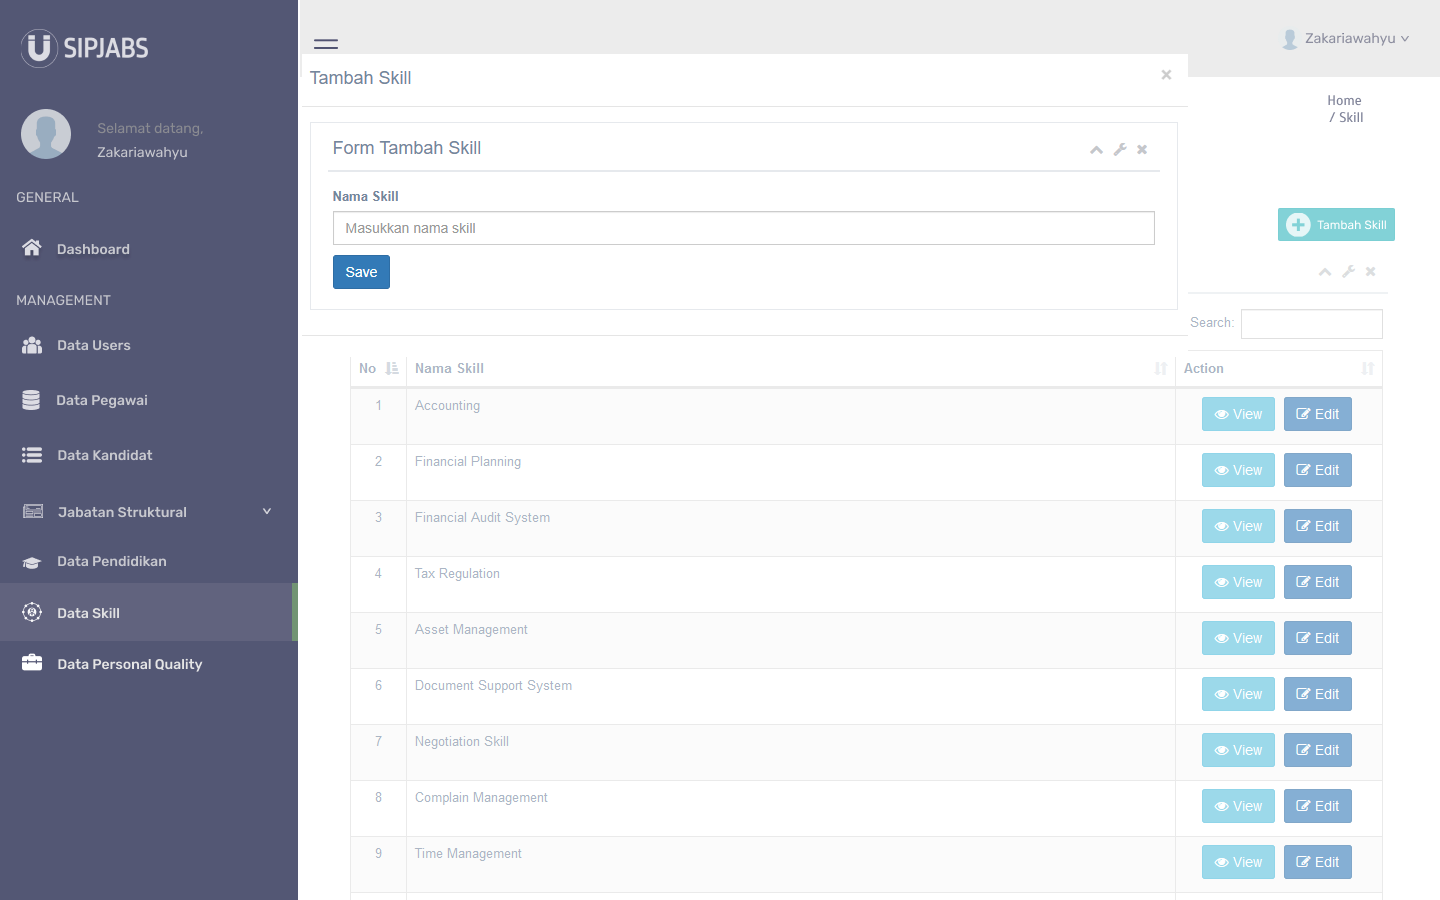
\includegraphics[width=0.6\textwidth, height=60mm]{pics/admin/tambahskill.png}} 
		& Admin dapat menambahkan data skill baru apabila terdapat data skill yang belum diinputkan.  \\
		
		\hline

		
	\end{tabular}
\end{table}

\subsubsection{Perancangan Antar Muka User}

\begin{table}
	\caption{Tabel Perancangan Antar Muka User}
	\centering
	\begin{tabular}{ | c | c | p{35mm} |}
		\hline 
		\textbf{No} & \textbf{Gambar} &  \textbf{Keterangan} \\ 
		\hline
		
		1. & \raisebox{-\totalheight}{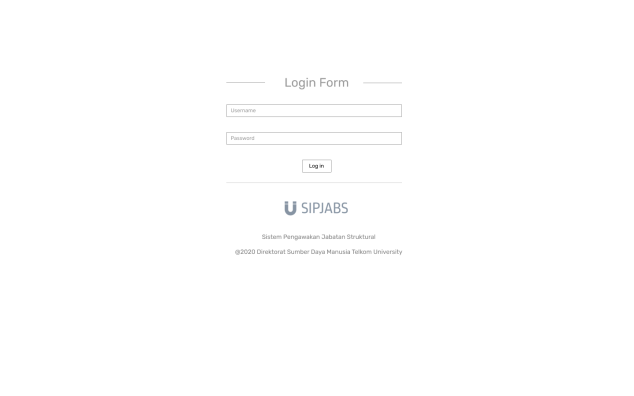
\includegraphics[width=0.6\textwidth, height=60mm]{pics/user/login.png}} 
		& Halaman login merupakan tampilan awal apabila user membuka aplikasi SiPJabS ,user dapat menginputkan username dan password untuk melakukan login.  \\
		
		\hline
		
		2. & \raisebox{-\totalheight}{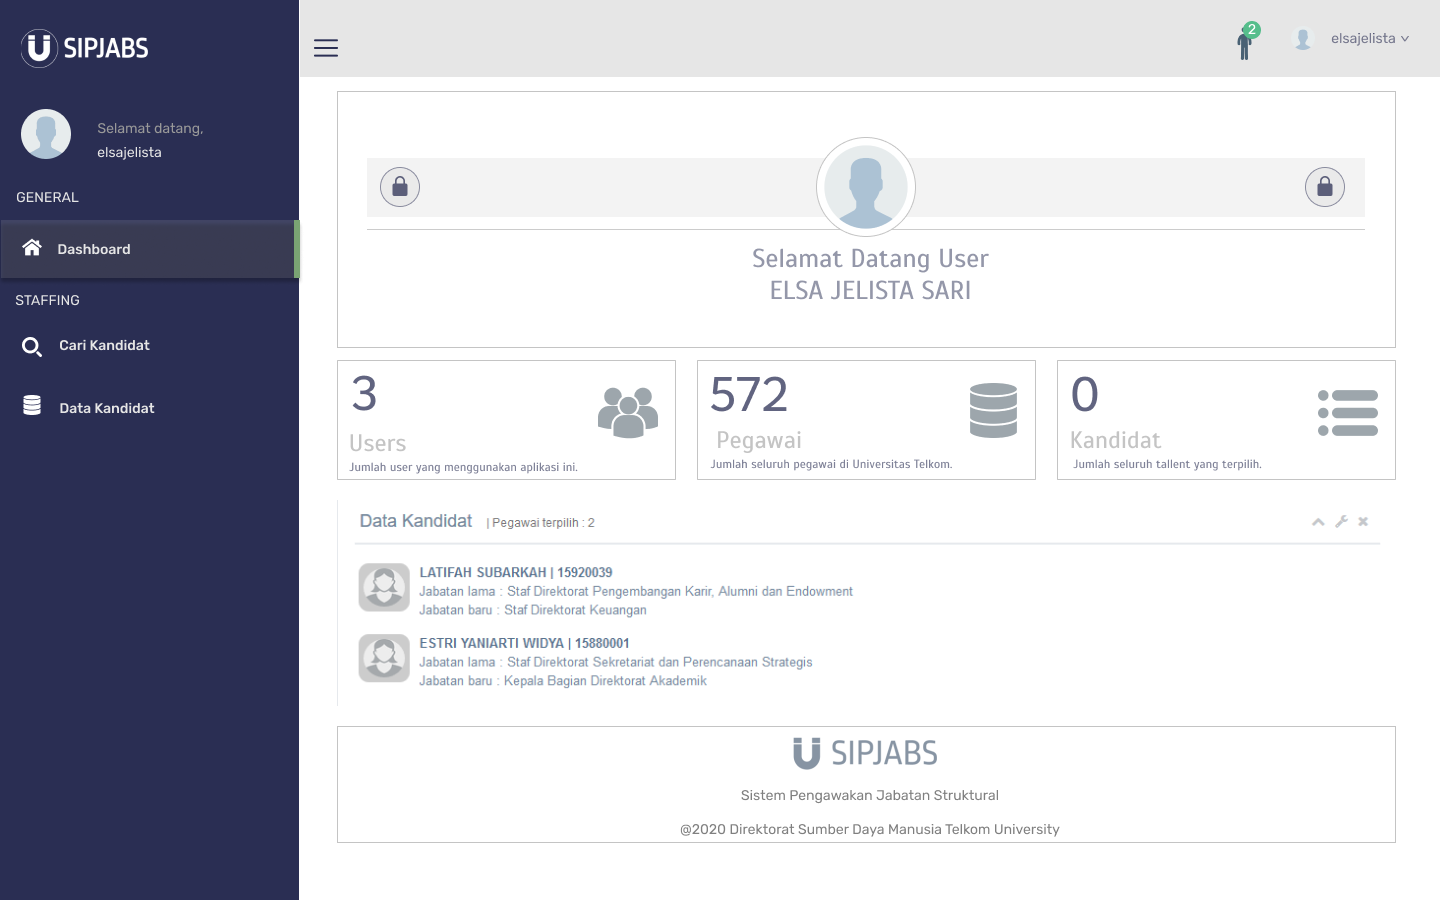
\includegraphics[width=0.6\textwidth, height=60mm]{pics/user/dashboard.png}} 
		& Halaman ini akan menampilkan jumlah user yang dapat mengakses aplikasi SiPJabS, jumlah pegawai yang ada di Universitas Telkom serta jumlah tallent yang sudah dipilih.  \\
		
		\hline
		
		3. & \raisebox{-\totalheight}{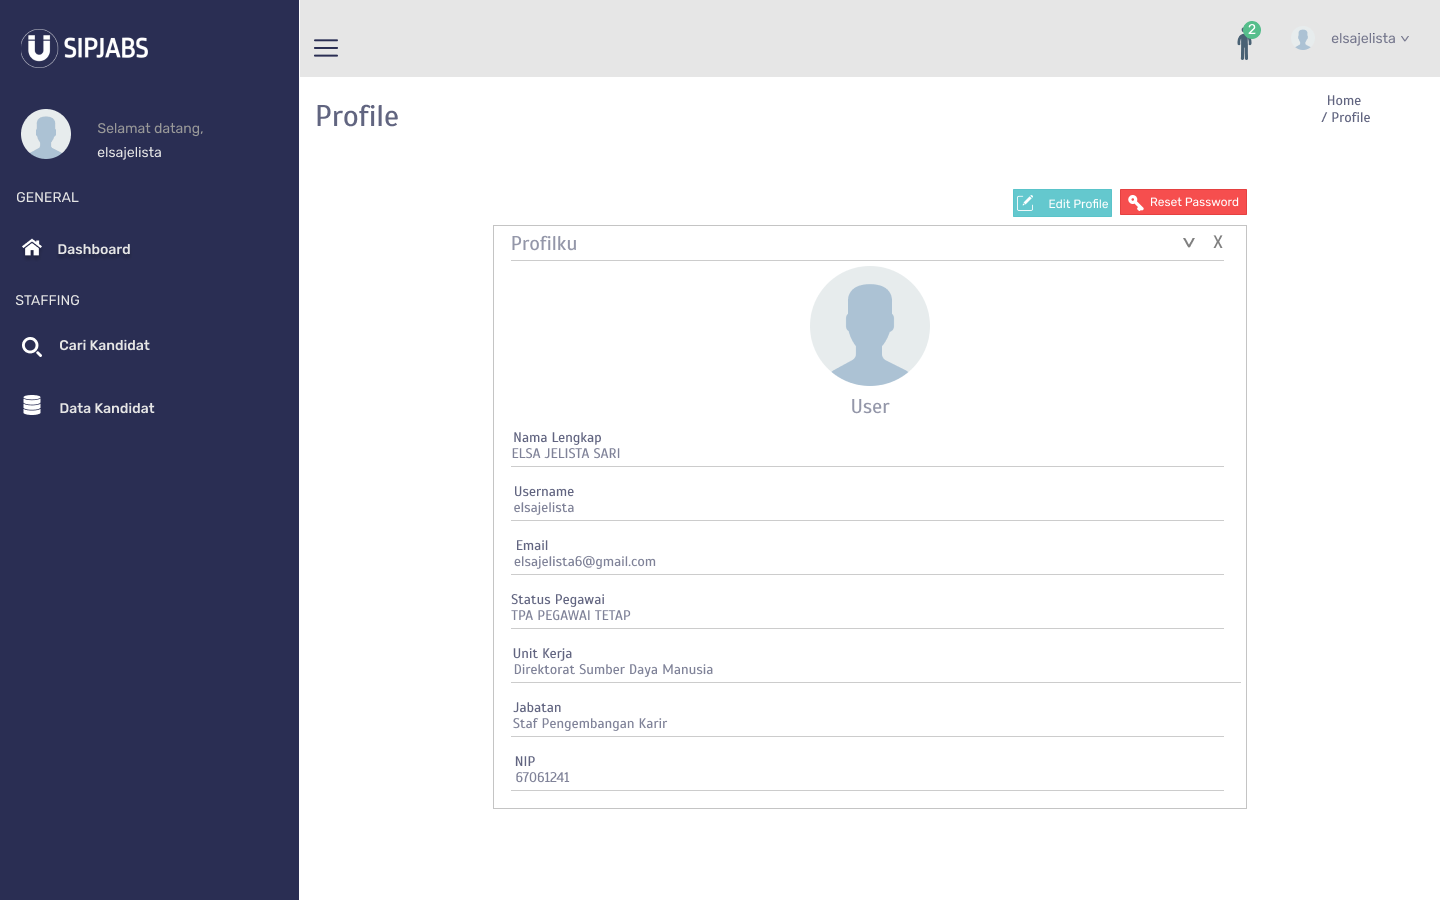
\includegraphics[width=0.6\textwidth, height=60mm]{pics/user/profile.png}} 
		& Halaman profile user akan menampilkan data nama lengkap, username, email, status pegawai, unit kerja, jabatan, serta NIP dari user tersebut. Kemudian user juga dapat mengedit profile dan mereset password.\\
		
		\hline
		
		
	\end{tabular}
\end{table}

\begin{table}
	\caption{Tabel Perancangan Antar Muka User (1)}
	\centering
	\begin{tabular}{ | c | c | p{35mm} |}
		\hline 
		\textbf{No} & \textbf{Gambar} &  \textbf{Keterangan} \\ 
		\hline
		
		4. & \raisebox{-\totalheight}{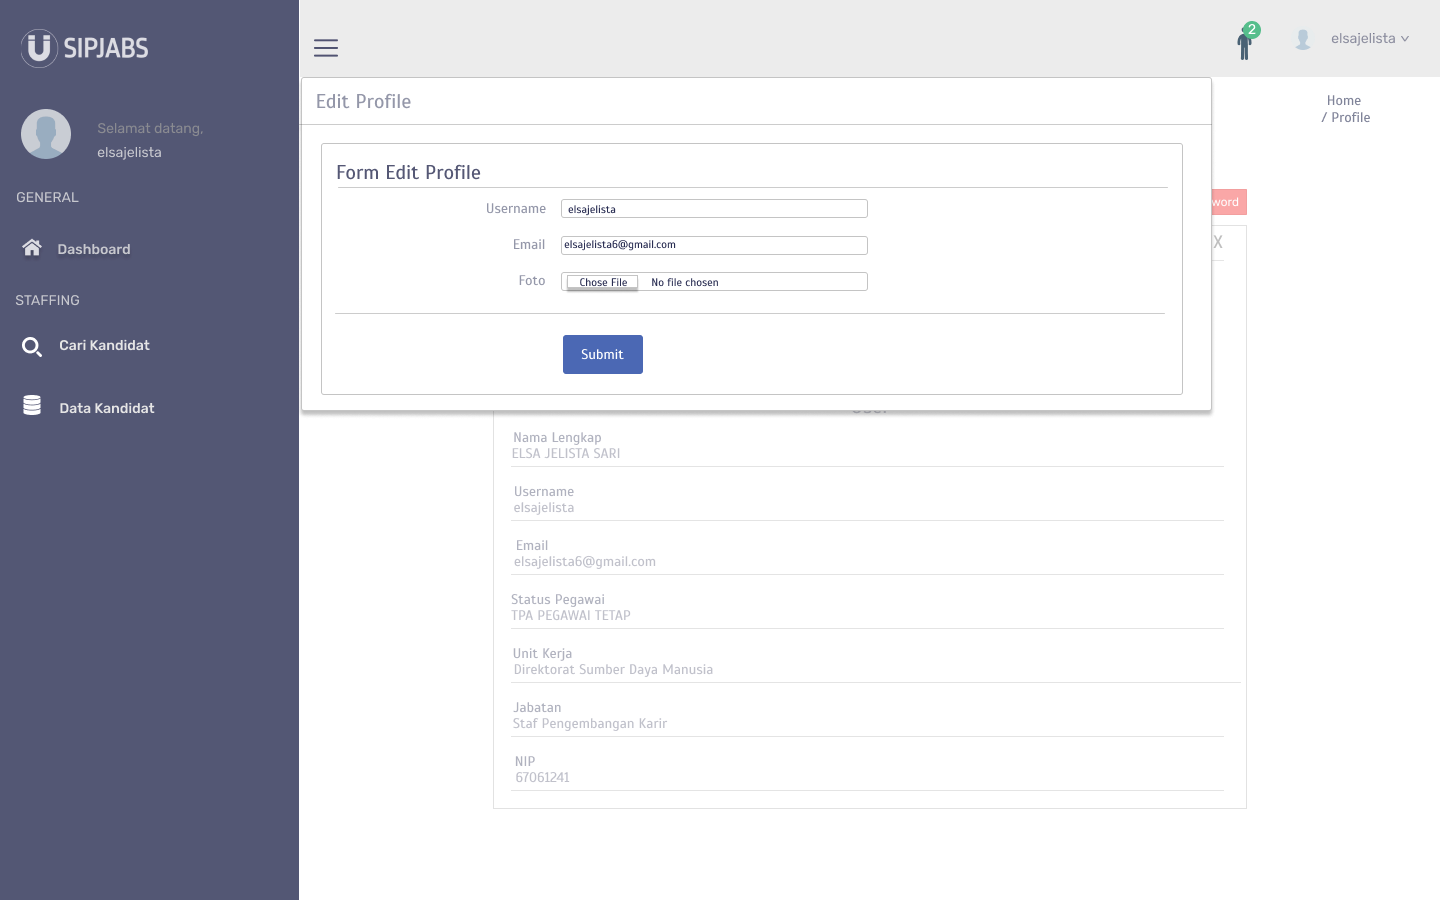
\includegraphics[width=0.6\textwidth, height=60mm]{pics/user/editprofile.png}} 
		& User dapat mengubah username, menginputkan email, dan menambahkan foto profile  \\
		
		\hline
		
		5. & \raisebox{-\totalheight}{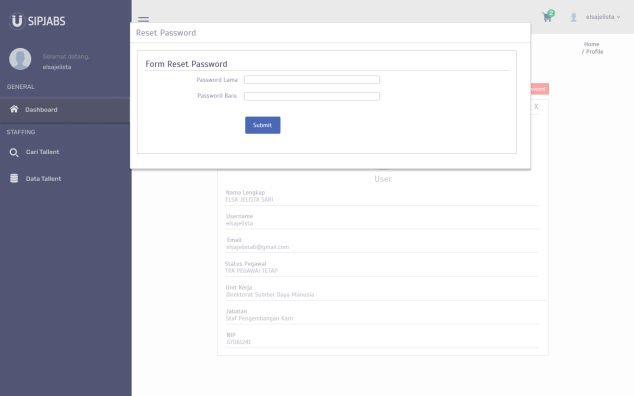
\includegraphics[width=0.6\textwidth, height=60mm]{pics/user/resetpassword.png}} 
		& User harus menginputkan password yang lama serta yang baru, setelah itu user dapat menyimpan.  \\
		
		\hline
		
		6. & \raisebox{-\totalheight}{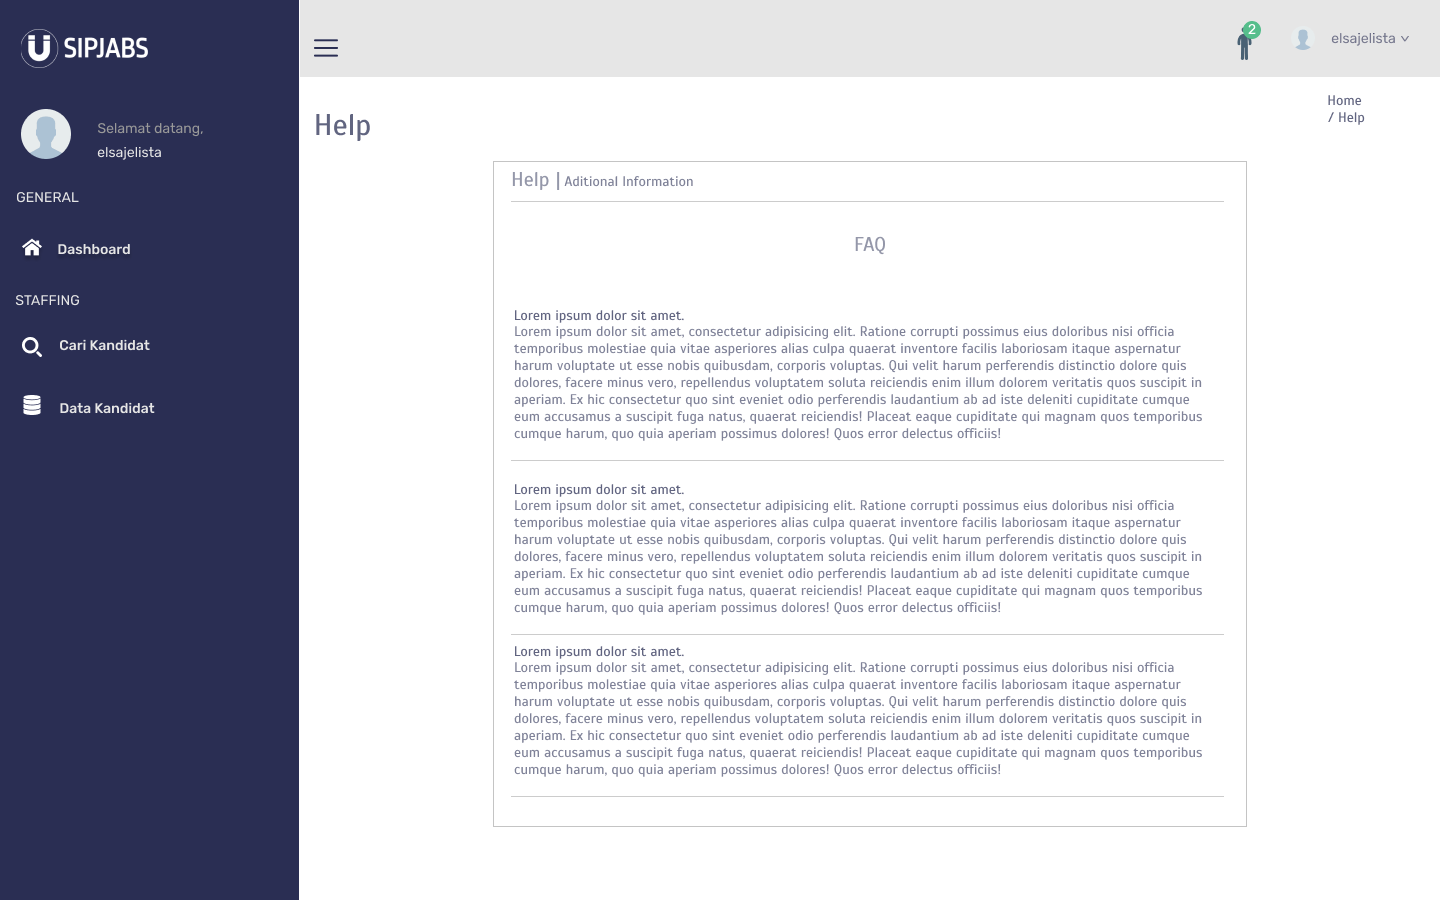
\includegraphics[width=0.6\textwidth, height=60mm]{pics/user/help.png}} 
		& Pada halaman help akan mengenai informasi dari sistem aplikasi ini\\
		
		\hline
		
	\end{tabular}
\end{table}

\begin{table}
	\caption{Tabel Perancangan Antar Muka User (1)}
	\centering
	\begin{tabular}{ | c | c | p{35mm} |}
		\hline 
		\textbf{No} & \textbf{Gambar} &  \textbf{Keterangan} \\ 
		\hline
		
		7. & \raisebox{-\totalheight}{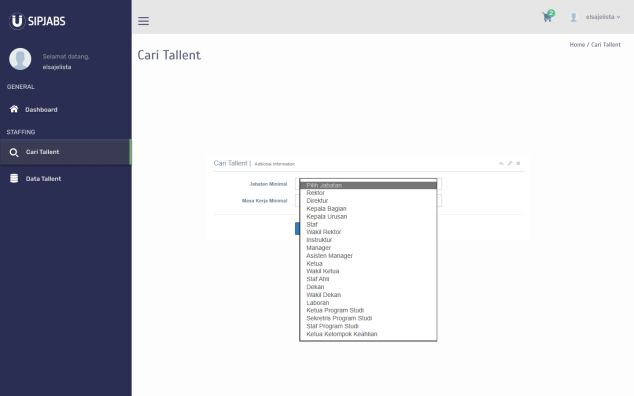
\includegraphics[width=0.6\textwidth, height=60mm]{pics/user/caritallent.png}} 
		& User dapat memilih jabatan dan masa kerja yang diinginkan untuk mengantikan atau mengisi posisi yang kosong.  \\
		
		\hline
		
		8. & \raisebox{-\totalheight}{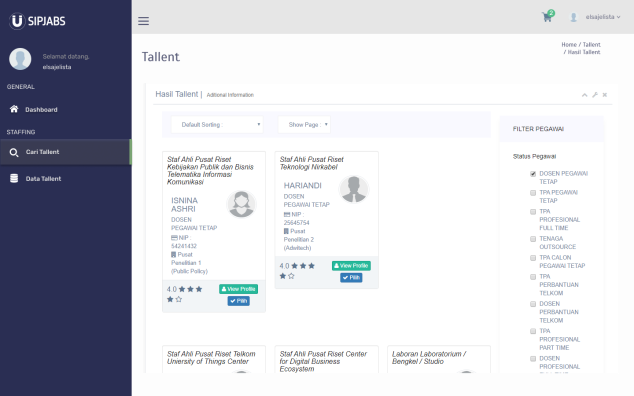
\includegraphics[width=0.6\textwidth, height=60mm]{pics/user/hasiltallent.png}} 
		& Halaman ini akan menampilkan tallent yang sudah di pilih dengan syarat tententu.   \\
		
		\hline
		
		9. & \raisebox{-\totalheight}{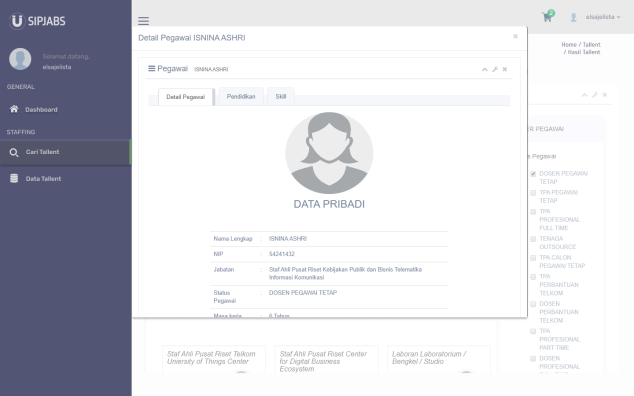
\includegraphics[width=0.6\textwidth, height=60mm]{pics/user/viewdetailtallent.png}} 
		& Halaman ini akan menampilkan data pribadi dari tallent tersebut.\\
		
		\hline
		
	\end{tabular}
\end{table}

\begin{table}
	\caption{Tabel Perancangan Antar Muka User (1)}
	\centering
	\begin{tabular}{ | c | c | p{35mm} |}
		\hline 
		\textbf{No} & \textbf{Gambar} &  \textbf{Keterangan} \\ 
		\hline
		
		10. & \raisebox{-\totalheight}{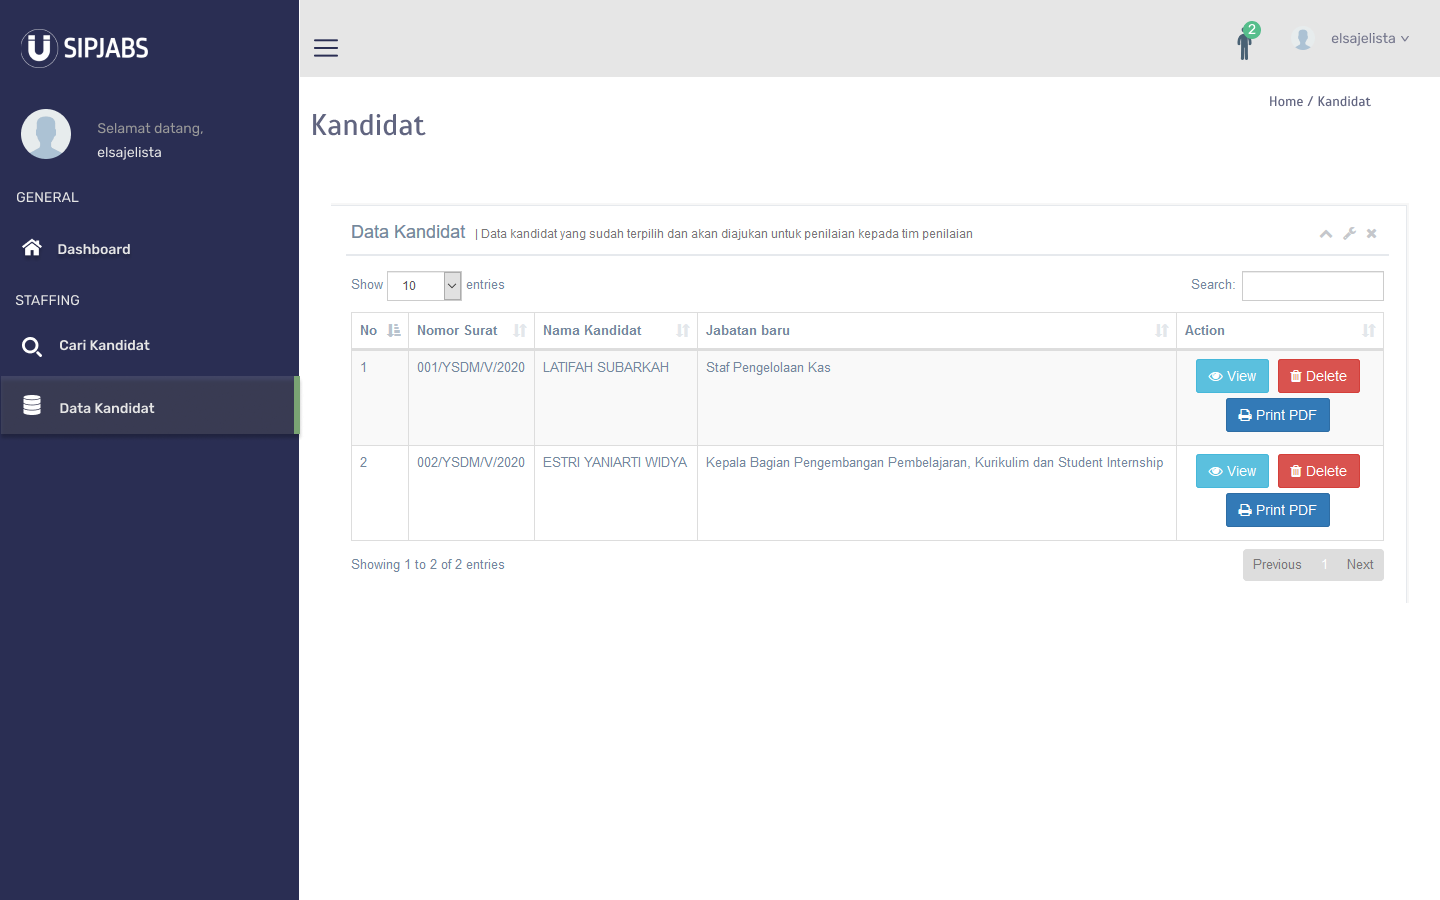
\includegraphics[width=0.6\textwidth, height=60mm]{pics/user/datatallent.png}} 
		& Halaman ini akan menampilkan data tallent yang sudah di proses dari cart tersebut.  \\
		
	
		\hline
		
	\end{tabular}
\end{table}
\subsection{Perancangan Level Tinggi}

\begin{figure}
	\centering
	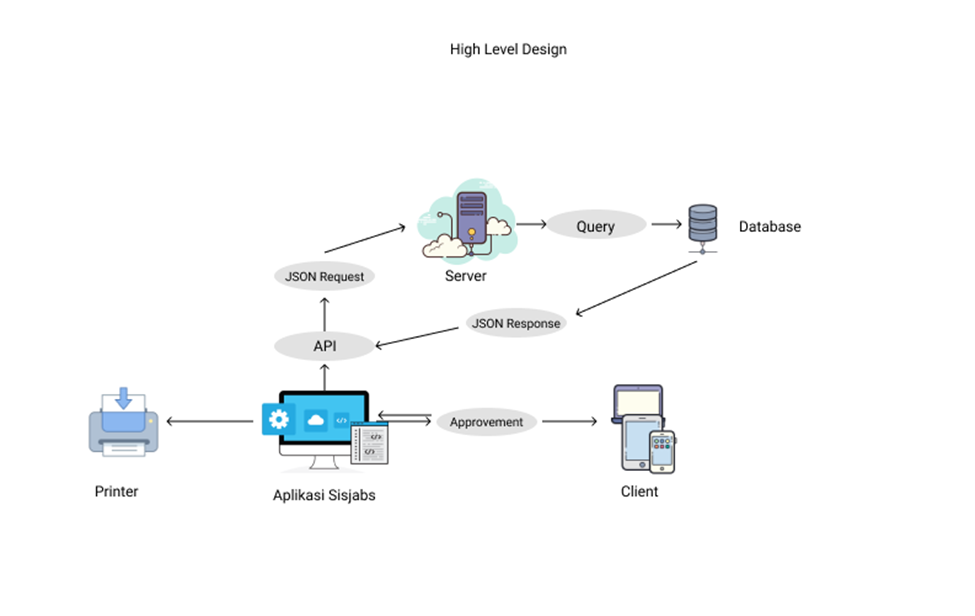
\includegraphics[width=0.9\textwidth]
	{pics/highleveldesign.png}
	\caption{High Level Design}
	\label{fig:34}
\end{figure}

Alur perancanaan level tinggi pada aplikasi pengawakan pegawai dimulai dari pengambilan API dalam bentuk JSON Request ke server. Pengambilan data akan di filter berdasarkan dengan query yang dibuat berdasarkan data yang diperoleh dari database yang ada. Kemudian database akan memberikan umpan balik berupa JSON Response berdasarkan request data yang akan ditampilkan kepada pengguna. 

